%%%%%%%%%%%%%%%%%%%%%%%%%%%%%%%%%%%%%%%%%%%%%%%%%%%%%%%%%%%%%%%%%%%%%%%%%%%%%%%%
% Preámbulo                                                                    %
%%%%%%%%%%%%%%%%%%%%%%%%%%%%%%%%%%%%%%%%%%%%%%%%%%%%%%%%%%%%%%%%%%%%%%%%%%%%%%%%

\documentclass[11pt,a4paper,titlepage,twoside,openright,openbib]{report}

%%% RELACIÓN DE VARIABLES A PERSONALIZAR %%%
%\def\lingua{gal}
\def\lingua{esp} % descomenta esta liña se redactarás a memoria en español
%\def\lingua{eng} % descomenta esta liña se redactarás a memoria en inglés
\def\nome{Welton Vieira dos Santos - welton.dossantos@udc.es}                             % substitúe aquí o teu nome
\def\nomeB{Pedro Pazos Curra - pedro.pazos@udc.es}                             % substitúe aquí o teu nome
\def\nomeC{Sergio Marcos Vázquez - sergio.marcosv@udc.es}                             % substitúe aquí o teu nome
\def\nomeD{Gabriel Alejandro Fernandéz Fernandéz - gabriel.fernandez1@udc.es}                             % substitúe aquí o teu nome
\def\nomedirectorA{Berta María Guijarro Berdiñas - berta.guijarro@udc.es}             % substitúe aquí o nome de quen dirixe
\def\titulo{Sistema inteligente de gestión logística de paquetería} % substitúe aquí o título do teu TFG
%\def\mencion{NOME DA MENCIÓN}                        % descomenta a mención correspondente
\def\mencion{COMPUTACIÓN}
%\def\mencion{ENXEÑARÍA DO SOFTWARE}
%\def\mencion{ENXEÑARÍA DE COMPUTADORES}
%\def\mencion{SISTEMAS DE INFORMACIÓN}
%\def\mencion{TECNOLOXÍAS DA INFORMACIÓN}

\def\renomearcadros{si} % descomenta esta liña se redactas a memoria en español e prefires que
                         % os "cuadros" e o "índice de cuadros" se renomeen
                         % a "tablas" e "índice de tablas" respectivamente

\usepackage{estilo_tfg}

% Lista de paquetes potencialmente interesantes (uso baixo demanda)

 \usepackage{alltt}       % proporciona o entorno alltt, semellante a verbatim pero que respecta comandos
 \usepackage{enumitem}    % permite personalizar os entornos de lista
 %\usepackage{eurofont}    % proporciona o comando \euro
 \usepackage{eurosym}    % proporciona o comando \euro
 \usepackage{float}       % permite máis opcións para controlar obxectos flotantes (táboas, figuras)
 \usepackage{hhline}      % permie personalizar as liñas horizontais en arrays e táboas
 \usepackage{longtable}   % permite construir táboas que ocupan máis dunha páxina
 \usepackage{lscape}      % permite colocar partes do documento en orientación apaisada
 \usepackage{moreverb}    % permite personalizar o entorno verbatim
 \usepackage{multirow}    % permite crear celdas que ocupan varias filas da mesma táboa
 \usepackage{pdfpages}    % permite insertar ficheiros en PDF no documento
 \usepackage{rotating}    % permite diferentes tipos de rotacións para figuras e táboas
 \usepackage{subcaption}  % permite a inclusión de varias subfiguras nunha figura
 \usepackage{tabu}        % permite táboas flexibles
 \usepackage{tabularx}    % permite táboas con columnas de anchura determinada

%%%%%%%%%%%%%%%%%%%%%%%%%%%%%%%%%%%%%%%%%%%%%%%%%%%%%%%%%%%%%%%%%%%%%%%%%%%%%%%%
% Corpo                                                                        %
%%%%%%%%%%%%%%%%%%%%%%%%%%%%%%%%%%%%%%%%%%%%%%%%%%%%%%%%%%%%%%%%%%%%%%%%%%%%%%%%

\begin{document}

 %%%%%%%%%%%%%%%%%%%%%%%%%%%%%%%%%%%%%%%%
 % Preliminares do documento            %
 %%%%%%%%%%%%%%%%%%%%%%%%%%%%%%%%%%%%%%%%

 \begin{titlepage}
  
  \hspace*{128pt}
  \textcolor{udcpink}{{\fontencoding{T1}\fontfamily{phv}\selectfont Facultade de Informática}}\\[-32pt]

  \begin{center}
    
\includegraphics[scale=0.3]{imaxes/udc}\\[35pt]

    {\large PRÁCTICAS DE DSI - 2022 \\
            GRADO EN INGENIERÍA INFORMÁTICA \\
            MENCIÓN EN \mencion } \\[100pt]
    
    \begin{huge}
      \begin{spacing}{1.3}
        \bfseries \titulo
      \end{spacing}
    \end{huge}
  \end{center}
  
  \vfill
  
  \begin{flushright}
    {\large
    \begin{tabular}{ll}
      {\bf Estudiantes:} & \nome \\
       & \nomeB \\
       & \nomeC \\
       & \nomeD \\
      {\bf Dirección:} & \nomedirectorA \\ % COPIA E PEGA ESTA LIÑA MÁIS VECES SE O PRECISAS
    \end{tabular}}
  \end{flushright}
  \rightline{A Coruña, \datasimple\today.}
\end{titlepage}

 \paxinaenbranco
 %\dedicatoria{Dedicatoria} % escribe neste comando o teu texto de dedicatoria
 %\paxinaenbranco
 %\paxinaenbranco
 %\begin{agradecementos}
 %\blindtext                % substitúe este comando polo teu texto de agradecementos
 %\end{agradecementos}
 %\paxinaenbranco
 %%%%%%%%%%%%%%%%%%%%%%%%%%%%%%%%%%%%%%%%%%%%%%%%%%%%%%%%%%%%%%%%%%%%%%%%%%%%%%%%%

\begin{abstract}\thispagestyle{empty}
  \blindtext % substitúe este comando polo resumo do teu TFG
             % na lingua principal do documento (tipicamente: galego)

  \vspace*{25pt}
  \begin{segundoresumo}
    \blindtext % substitúe este comando polo resumo do teu TFG
               % na lingua secundaria do documento (tipicamente: inglés)
  \end{segundoresumo}
\vspace*{25pt}
\begin{multicols}{2}
\begin{description}
\item [\palabraschaveprincipal:] \mbox{} \\[-20pt]
  \blindlist{itemize}[7] % substitúe este comando por un itemize
                         % que relacione as palabras chave
                         % que mellor identifiquen o teu TFG
                         % no idioma principal da memoria (tipicamente: galego)
\end{description}
\begin{description}
\item [\palabraschavesecundaria:] \mbox{} \\[-20pt]
  \blindlist{itemize}[7] % substitúe este comando por un itemize
                         % que relacione as palabras chave
                         % que mellor identifiquen o teu TFG
                         % no idioma secundario da memoria (tipicamente: inglés)
\end{description}
\end{multicols}

\end{abstract}

%%%%%%%%%%%%%%%%%%%%%%%%%%%%%%%%%%%%%%%%%%%%%%%%%%%%%%%%%%%%%%%%%%%%%%%%%%%%%%%%

 %\paxinaenbranco

 \pagenumbering{roman}
 \setcounter{page}{1}
 \bstctlcite{IEEEexample:BSTcontrol}

 \tableofcontents
 \listoffigures
 \listoftables
 \lstlistoflistings 	    % Índice de códigos
 \cleardoublepage
 
 \pagenumbering{arabic}
 \setcounter{page}{1}

 %%%%%%%%%%%%%%%%%%%%%%%%%%%%%%%%%%%%%%%%
 % Capítulos                            %
 %%%%%%%%%%%%%%%%%%%%%%%%%%%%%%%%%%%%%%%%

% \chapter{Introdución}
\label{chap:introducion}

\lettrine{P}{rimer} capítulo da memoria, onde xeralmente se exporán as
liñas mestras do traballo, os obxectivos, etc. Incluimos un par de
exemplos de citas~\cite{ErlangBook,ErlangWebBook} e de referencias
internas (sección \ref{sec:mostra}, páxina \pageref{sec:mostra}).

\Blindtext

\section{Sección de mostra}
\label{sec:mostra}

\Blindtext

\subsection{Subsección de mostra}

\Blindtext

% \chapter{Contido demostrativo}
\label{chap:demo}

\lettrine{E}{ntre} a introdución e as conclusións, o documento conterá
tantos capítulos como sexa preciso, sempre con coidado de non rebasar
o límite de 80 páxinas fixado polo regulamento de TFGs.

Empregaremos éste de xeito demostrativo, para ilustrar o uso de
elementos habituais que poidan ser de utilidade\footnote{Por exemplo,
  isto é unha nota a pé de páxina.}.

\section{Inclusión de imaxes}

Se precisamos imaxes no noso documento, incluirémolas do xeito que se
indica na figura~\ref{fig:exemplo} (páxina~\pageref{fig:exemplo}). Se
o facemos así, \LaTeX ubicará cada imaxe no mellor lugar posible,
lugar que pode variar a medida que o documento vaia crecendo coa
inclusión de máis texto e outros elementos (máis imaxes, táboas,
etc.).

\begin{figure}[hp!]
  \centering
  
\includegraphics[width=0.75\textwidth]{imaxes/udc.png}
  \caption{Pé de imaxe descritivo}
  \label{fig:exemplo}
\end{figure}

Recoméndase almacenar os ficheiros gráficos no directorio
\texttt{imaxes}.

\subsection{Inclusión de varias sub-imaxes}

Se precisamos inserir imaxes relacionadas, pode ser apropiado
incluílas como sub-figuras, do xeito que se pode apreciar na
figura~\ref{fig:exemplo-subfiguras} coas
imaxes~\ref{fig:subfigura-rotada}
e~\ref{fig:subfigura-deformada}. Como se pode ver nos exemplos desta
sección, sempre é recomendable referirse ás imaxes pola súa
referencia, xa que dese xeito non dependemos de onde queden ubicados
os elementos en cuestión.

\begin{figure}[hp!]
  \centering
  \begin{subfigure}[c]{0.3\textwidth}
    
\includegraphics[angle=45,width=\textwidth]{imaxes/udc.png}
    \caption{Pé de subimaxe rotada}
    \label{fig:subfigura-rotada}
  \end{subfigure}
  \hspace{0.1\textwidth}
  \begin{subfigure}[c]{0.3\textwidth}
    
\includegraphics[width=\textwidth,height=3cm]{imaxes/udc.png}
    \caption{Pé de subimaxe deformada}
    \label{fig:subfigura-deformada}
  \end{subfigure}
  \caption{Pé de imaxe xeral}
  \label{fig:exemplo-subfiguras}
\end{figure}

\section{Inclusión de código fonte}

Se precisamos incluír fragmentos de código fonte, podemos facelo da
seguinte maneira:

\begin{lstlisting}[language=PYTHON]
#include <stdio.h>
#define N 10

int main()
{
  int i;

  // Isto é un comentario
  puts("Ola, mundo!");

  for (i = 0; i < N; i++)
  {
    puts("LaTeX é a ferramenta de edición ideal para profesionais da informática!");
  }

  return 0;
}
\end{lstlisting}

\section{Uso da relación de acrónimos e do glosario}

Os acrónimos edítanse no ficheiro \texttt{bibliografia/acronimos.tex}
e úsanse empregando a orde \texttt{acrlong} para obter o termo
completo (deste xeito: \acrlong{erlang}), a orde \texttt{acrshort}
para obter o acrónimo (deste xeito: \acrshort{erlang}). A primeira vez
que usamos un termo con acrónimo no documento é recomendable usar orde
\texttt{acrfull} (que produce ambas versións á vez:
\acrfull{erlang}). Os acrónimos que non se usan no documento, non
aparecen na relación que se xerar na versión PDF.

Pola súa banda, os termos do glosario edítanse no ficheiro
\texttt{bibliografia/glo\-sa\-rio.tex} e úsanse empregando a orde
\texttt{gls} (deste xeito, \gls{bytecode}) ou \texttt{Gls} (deste
xeito, \Gls{bytecode}). Ao igual que os acrónimos, os termos que non
se usan no documento, non aparecen na relación que se xera na versión
PDF.

%\include{contido/...}
% \chapter{Conclusións}
\label{chap:conclusions}

\lettrine{D}{erradeiro} capítulo da memoria, onde se presentará a
situación final do traballo, as leccións aprendidas, a relación coas
competencias da titulación en xeral e a mención en particular,
posibles liñas futuras,\dots

\Blindtext

%%%%%%%%%%%%%%%%%%%%%%%%%%%%%%%%%%%%%%%%%%%%%%%%%%%%%%%%%%%%%%%%%%%%%%%%
% Plantilla TFG/TFM
% Universidad de A Coruña. Facultad de Informática
% Realizado por: Welton Vieira dos Santos
% Modificado: Welton Vieira dos Santos
% Contacto: welton.dossantos@udc.es
%%%%%%%%%%%%%%%%%%%%%%%%%%%%%%%%%%%%%%%%%%%%%%%%%%%%%%%%%%%%%%%%%%%%%%%%


\chapter{Análisis de Viabilidad: Modelado de la Organización.}

\newpage
\section{Formulario OM-1: Contexto Organizacional, problemas y soluciones.}
Identificación de los problemas y oportunidades orientadas al conocimiento de la organización, como se muestra en la Tabla \ref{tab:OM1}.


\begin{table}[H]
  \scriptsize
  \resizebox{15,0cm}{!}{
    \begin{tabularx}{\textwidth}{|l|X|} 
      \hline
      \textbf{Modelo de Organización} & \textbf{Formulario OM-1: Problemas y Posibilidades de Mejora} \\ 
      \hline
      \hline
      \textsc{Problemas y Oportunidades} & El conjunto de medios y/o métodos necesarios para llevar a cabo la organización de una empresa, también conocido como logística, tiene una gran relevancia en la misma. Hemos sido contratados por una empresa de paquetería en España (MRW), con el objetivo de desarrollar un sistema inteligente para mejorar su forma de gestionar los recursos de entrega y recogida de paquetería. Si bien es cierto que esta tarea requiere de un conocimiento adquirido mediante la experiencia, su reiteratividad en muchos aspectos facilita una posible automatización. Actualmente, MRW carece de herramienta o sistema que facilite la tarea de asignación de recursos, lo cual, tiene una serie de implicaciones:
      \begin{enumerate}
        \item Se depende completamente de la capacidad de decisión y el rendimiento del personal asignado a la tarea de asignación.
        \item Al depender únicamente del recurso humano, el registro de cómo han sido asignados los paquetes no es automatizable, se debe realizar manualmente.
        \item La solución proporcionada por el personal asignado, en muchos casos, difiere de la óptima o de una próxima a la mejor posible.
      \end{enumerate}\\ 
      \hline
      \textsc{Contexto Organizacional} & 
      MRW es una importante empresa de paquetería y logística con envíos internacionales de paquetes de diversos tipos, cuya partida hay que planificar, dando continuidad al sistema de automación de la logística de la empresa, que ya cuenta con un sistema de prioridad de entrega según la ruta asignada con el fin de lograr correctamente el cometido: maximizar los recursos que posee la empresa para gestionar las paqueterías que se recibe por parte de la central de MRW con el propósito de entregar/recoger el mayor número de paquetes en el menor tiempo y coste posibles. 

      Dicha organización se rige por la obtención del máximo beneficio de la gestión de la paquetería que la franquicia pueda obtener, mientras brinda la mejor calidad del servicio que pueda ofrecer a sus clientes. Además, los valores diferenciales 
      con los que identifican son la fiabilidad, calidad, rapidez, innovación, capilaridad, sostenibilidad y cercanía.

      La empresa cuenta con 550 franquicias y 58 plataformas logísticas en Andorra, España, Gibraltar y Portugal y realiza una media de 70 millones de envíos anuales. Su modelo organizativo se divide en diversos departamentos con funciones claramente diferenciadas (Facturación, Atención al cliente, Logística, Comercial, RR.HH) \\ 
      \hline
      \textsc{Soluciones} & La solución que se propone es desarrollar un sistema que pueda calcular de forma inteligente y óptima los recursos que posee la empresa, es decir, optimizar la gestión de los paquetes que cada vehículo pueda llevar. \\
      \hline
    \end{tabularx}
  }
  \caption{\label{tab:OM1}Contexto Organizacional - OM1}
\end{table}
	
 
%%%%%%%%%%%%%%%%%%%%%%%%%%%%%%%%%%%%%%%%%%%%%%%%%%%%%%%%%%%%%%%%%%%%%%%%%%%%%%%
\section{Formulario OM-2: descripción del área de interés de la organización.}

Descripción de los aspectos de la organización que tienen impacto y/o se ven afectados
  por las soluciones basadas en conocimiento elegidas.


\begin{table}[H]
  \scriptsize
  \resizebox{14,0cm}{!}{
    \begin{tabularx}{\textwidth}{|l|X|} 
      \hline
      \textbf{Modelo de Organización} & \textbf{Formulario OM-2: Aspectos Variables} \\ 
      \hline
      \hline
      \textsc{Estructura} & La organización de la empresa MRW se puede ver en la figura (Figura \ref{fig:diagramaEstructura}), donde se puede observar un primer departamento encargado de la dirección del resto de departamentos (Facturación, Atención al cliente, Logística, Comercial y Recursos Humanos). \\ &
      \begin{itemize}
        \item Facturación: Departamento encargado de emitir y entregar factura por las actividades realizadas en el desarrollo de la actividad empresarial.
        \item Atención al cliente: Departamento encargado de la atención al cliente, donde esos clientes pueden recoger o entregar paquetes in situ.
        \item Logística: Departamento encargado de todas las actividades relacionadas con la distribución, tanto de los paquetes como de los envíos de la propia paquetería.
        \item Comercial: Departamento encargado de dar a conocer los productos o servicios que comercializa la empresa a través de acciones publicitarias y de promoción, de actualizar los productos en función de las necesidades y cambios en el mercado o de gestionar las relaciones con los clientes.
        \item Recursos Humanos: Departamento encargado de la gestión de los recursos humanos de la organización.
      \end{itemize} \\ 
      \hline
      \textsc{Procesos} & El proceso de distribución de la paquetería se puede descomponer en 4 fases principales: 
      \begin{enumerate}
        \item Recibimiento de los paquetes en la sucursal MRW (entrada).
        \item Generar lista de entregas según ruta asignada.
        \item Determinar los recursos disponibles por la sucursal MRW para entregar según ruta (paquete, personal, transporte, rutas de transporte).
        \item Revisión y validación de la distribución de la paquetería.
      \end{enumerate} \\ 
      \hline
      \textsc{Personal} &  Los trabajadores encargados de escanear los paquetes para otorgar al sistema información de los mismos y aquellos encargados de repartir en los vehículos (repartidores) pueden o no ser los mismos. Toda la plantilla estaría conformada de trabajadores desde baja cualificación en adelante (sin restricción).

      Además, estos estarán liderados por un director. \\ 
      \hline
      \textsc{Recursos} &  Describir los recursos utilizados por los procesos:
      \begin{enumerate}
          \item Sistemas de información y otros recursos computacionales:
          \begin{enumerate}
            \item Sistema inteligente.
            \item Base de datos de paquetes.
            \item Base de datos de flota de vehículos.
          \end{enumerate}
          \item Equipamiento y material.
          \begin{enumerate}
            \item Infraestructura informática (escáneres, teléfonos móviles).
            \item Conexión a Internet.
          \end{enumerate}
      \end{enumerate} \\ 
      \hline
      \textsc{Conocimiento} &  Experto/s en logística especializado/s en la distribución de paquetería \\ 
      \hline
      \textsc{Cultura y Potencial} &  Los colaboradores de la empresa tiene funciones específicas, es decir, hay una persona que se encarga de la atención al cliente, otra persona se encarga de gestionar la logística y los repartidores se encargan de efectuar la entrega/recogida de la paquetería según la ruta asignada por logística. La comunicación, cordialidad y el respeto mutuo es la tónica más importante para el desarrollo de la actividad. \\ 
      \hline
    \end{tabularx}
  }
  %\label{tab.OM2}
  \caption{\label{tab:OM2}Descripción del área de interés de la organización - OM2}
\end{table}

\begin{figure}[H]
	\centering
	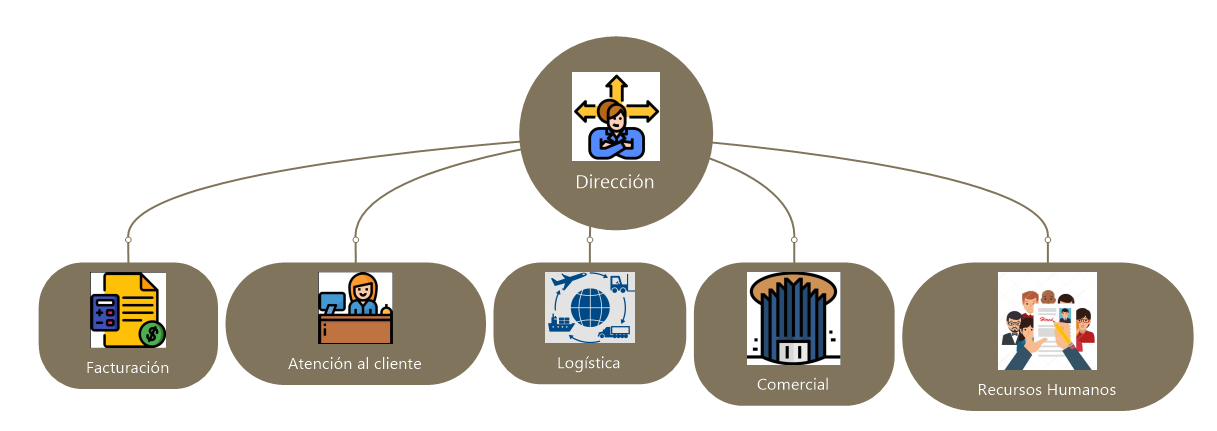
\includegraphics[scale=0.50]{imaxes/Organigrama.png}
	\caption{\label{fig:diagramaEstructura}Diagrama estructura - Formulario OM2}
\end{figure}

\section{Formulario OM-3: Descomposición del Proceso de Negocio.}

Descripción del proceso de interés a partir de las tareas que lo componen.

\begin{table}[H]
  \centering
  \resizebox{15,0cm}{!}{
    \begin{tabular}{|c|c|c|c|c|c|c|}
      \hline
      \multicolumn{3}{|c}{\textbf{Modelo de Organización}} & \multicolumn{4}{|c|}{\textbf{Formulario OM-3: Descomposición de los Procesos}}\\
      \hline \hline
      \textsc{N\textordmasculine} & \textsc{Tarea} & \textsc{Realiza\-da por} & \textsc{¿Dónde?} & \textsc{Recursos de Conocimiento} & \textsc {¿In\-ten\-si\-va en Conocimiento?} & \textsc{Im\-por\-tan\-cia} \\
      \hline

      1 & Recibimiento de los paquetes en la sucursal MRW (entrada) & \multicolumn{1}{|p{3.0cm}|}{\centering Repartidor experimentado} & \multicolumn{1}{|p{3.0cm}|}{\centering En la nave de la sucursal de MRW} & \multicolumn{1}{|p{5.0cm}|}{\centering No } & No & Requisito necesario para iniciar el proceso \\
      \hline
      2 & Generar lista de entregas según ruta asignada & \multicolumn{1}{|p{3.0cm}|}{\centering Repartidor experimentado} & \multicolumn{1}{|p{3.0cm}|}{\centering En la nave de la sucursal de MRW} & \multicolumn{1}{|p{5.0cm}|}{\centering Experiencia en reparto de paquetes según la ruta asignada} & Sí (bajo) & Máxima \\
      \hline
      3 & Determinar los recursos disponibles por la sucursal MRW para entregar según ruta & \multicolumn{1}{|p{3.0cm}|}{\centering Equipo Directivo, Repartidor experimentado} & \multicolumn{1}{|p{3.0cm}|}{\centering En la nave de la sucursal de MRW} & \multicolumn{1}{|p{5.0cm}|}{\centering Experiencia en distribución de recursos. Utilizar teoria de programación dinámica} & Sí (elevado) & Máxima \\
      \hline
      4 & Revisión y validación de la distribución de la paquetería & \multicolumn{1}{|p{3.0cm}|}{\centering Equipo Directivo} & \multicolumn{1}{|p{3.0cm}|}{\centering En la nave de la sucursal de MRW} & \multicolumn{1}{|p{5.0cm}|}{\centering Experiencia en distribución de recursos. Utilizar teoria de programación dinámica} & Moderado & Recomendable \\
      \hline      
    \end{tabular}
  }
	\caption{\label{tab:OM3}Descomposición del proceso de negocio - OM3}
\end{table}

\newpage
\section{Formulario OM-4: Activos de Conocimiento}
%%%%%%%%%%%%%%%%%%%%%%%%%%%%%%%%%%%%%%%%%%%%%%%%%%%%%%%%%%%%%%%%%%%%%%%%%%%%%%%

Descripción del componente \textit{conocimiento} del modelo de la organización.

\begin{table}[H]
  \centering
  \resizebox{15,0cm}{!}{
    \begin{tabular}{|c|c|c|c|c|c|c|}
      \hline
      \multicolumn{3}{|c}{\textbf{Modelo de Organización}} & \multicolumn{4}{|c|}{\textbf{Formulario OM-4: Activos de Conocimiento}}\\
      \hline \hline
      \textsc{Recurso de Conocimiento} & \textsc{Pertenece} & \textsc{Usado en} & \textsc{¿Forma Cor\-recta?} & \textsc{¿Lugar Cor\-recto?} & \textsc {¿Tiempo Cor\-recto?} & \textsc{¿Calidad Cor\-recta?} \\
      \hline
      
      \multicolumn{1}{|p{4.0cm}|}{\centering Experiencia en reparto de paquetes según la ruta asignada} & \multicolumn{1}{|p{3.0cm}|}{\centering Expertos en reparto} & \multicolumn{1}{|p{3.0cm}|}{\centering Tarea 2 de OM-3} & \multicolumn{1}{|p{3.0cm}|}{\centering Si, el conocimiento se puede adquirir con sistema de ubicación por código postal.} & Departamento de logística & - & \multicolumn{1}{|p{3.0cm}|}{\centering Sí, teniendo en cuenta que son aproximaciones} \\      
      \hline
      \multicolumn{1}{|p{4.0cm}|}{\centering Experiencia en distribución de recursos/ Utilizar teoria de programación dinámica} & \multicolumn{1}{|p{3.0cm}|}{\centering Experto (director) y equipo directivo} & \multicolumn{1}{|p{3.0cm}|}{\centering Tarea 3 y 4 de OM-3} & \multicolumn{1}{|p{3.0cm}|}{\centering Si, el conocimiento se puede adquirir con las teorías de programación dinámica} & Departamento de logística & - & \multicolumn{1}{|p{3.0cm}|}{\centering Sí, teniendo en cuenta que son aproximaciones} \\      
      \hline
    \end{tabular}
  }
	\caption{\label{tab:OM4}Activos de conocimiento - OM4}
\end{table}


\section{Formulario OM-5: Análisis de viabilidad}


Elementos a considerar en el análisis de la viabilidad del proyecto. Nota: para mayor comodidad, en este apartado se puede prescindir del formato ``tabla'' y transformarla en subsecciones (comando subsubsection) manteniendo los mismos epígrafes de la primera columna.

\begin{table}[H]
  \centering
  \resizebox{15.0cm}{!}{
    \begin{tabular}{|l|l|} 
      \hline
      \textbf{Modelo de Organización} & \textbf{Formulario OM-5: Elementos del Documento de Viabilidad}\\ 
      \hline
      \hline

      \textsc{Viabilidad Empresarial} & \multicolumn{1}{p{14.0cm}|}{
      Al sustituir el trabajo de obra manual por un sistema automatizado; aumenta significativamente la velocidad en la tarea de asignación, lo cual supone también una reducción del coste, concretamente se reduce un 40\% el coste de mano de obra a principio de la jornada, además, al tener un sistema más preciso se evitan confusiones en la asignación.\newline
      Para llevar a cabo la implantación del sistema inteligente, la sucursal necesitará hacer una gran inversión: 
      \begin{itemize}
        \item Dos analistas durante cinco días (una semana) en una jornada completa (8 horas). Costo de $7.5 €/h$ con un total estimado de $600.00€$
        \item Cuatro desarrolladores trabajando diez días laborables (dos semanas) a jornada completa (8 horas). Costo de $7.5 €/h$ con un total estimado de $2400.00€$
        \item Un tester trabajando trabajando diez días (dos semanas) laborables a jornada completa (8 horas). Costo de $7.5 €/h$ con un total estimado de $600.00€$
        \item Dos técnicos trabajando cinco días laborables (una semana) a jornada completa (8 horas).Costo de $7.5 €/h$ con un total estimado de $600.00€$
        \item Empresa subcontratada para realizar la instalación de una cinta transportadora que garantiza la realización del trabajo en dos semanas.Costo total estimado de $10000.00€$ con todo el material incluido.
      \end{itemize}
      
      El proyecto no cambiaría el organigrama de la empresa ya que la parte que se hacía de forma manual ahora se hará de forma más automática, sin la necesidad de añadir/excluir algún departamento.

      Es un proyecto de riesgo bajo para el capital inicial invertido en ese proyecto, puesto que no afectará el funcionamiento de la empresa, ya que la misma ya se encuentra operativa y recibiendo beneficios de su operativa diaria.}\\
      \hline
    \end{tabular}
  }
  \caption{\label{tab:OM5}Formulario OM-5 (Parte 1). Viabilidad Empresarial}
\end{table}

\begin{table}[H]
  \centering
  \resizebox{15.0cm}{!}{
    \begin{tabular}{|l|l|} 
      \hline
      \textbf{Modelo de Organización} & \textbf{Formulario OM-5: Elementos del Documento de Viabilidad}\\ 
      \hline
      \hline

      \textsc{Viabilidad Técnica} & \multicolumn{1}{p{14.0cm}|}{
      La tarea a realizar tiene una baja complejidad técnica en el aspecto de conocimiento pues los problemas que se resolverán tienen una baja carga computacional para el sistema.\newline
      No hay impedimentos críticos de recursos o de tiempo, pues la empresa ya tiene su propia metodología en funcionamiento y suficientes ingresos como para evaluar la elaboración del proyecto con todos los recursos necesarios. \newline
      El éxito del proyecto estará determinado por la mejora en la calidad del servicio, la eficiencia de las entregas y en la satisfacción de todos los agentes involucrados en el mismo con la solución proporcionada. \newline
      La interacción con los usuarios finales del sistema (empleados de MRW) será sencilla y sin complejidad, prácticamente llevarán a cabo sus tareas rutinarias excepto las automatizadas por el sistema, además, los últimos (y futuros) avances en materia de accesibilidad a la tecnología y facilidad de uso, permitirán una usabilidad muy sencilla con nuestro sistema. \newline
      La interacción de este sistema con otros no sería complejo debido a que maneja fuentes de datos fácilmente parseables y flexibles (sistema de gestión de bases de datos que almacena datos de paquetes, flota, empleados y rutas). \newline
      El sistema no supodría un riesgo asociado a hipotéticos cambios tecnológicos en el futuro así como también posibles cambios en la legislación vigente sobre la protección datos.
      } \\
      \hline
    \end{tabular}
  }
  \caption{\label{tab:OM5-2}Formulario OM-5 (Parte 2). Viabilidad Técnica}
\end{table}

\begin{table}[H]
  \centering
  \resizebox{15.0cm}{!}{
    \begin{tabular}{|l|l|} 
      \hline
      \textbf{Modelo de Organización} & \textbf{Formulario OM-5: Elementos del Documento de Viabilidad} \\ 
      \hline
      \hline

      \textsc{Viabilidad del Proyecto} & \multicolumn{1}{p{14.0cm}|}{
        Con probabilidad hay un interés más que suficiente en la elaboración del proyecto debido a que podrá abaratar en gran medida los costes del proceso logístico de la empresa. \newline
        Los recursos están disponibles con facilidad debido a que la empresa ya está haciendo uso de la mayor parte de ellos y ya dispone de lo necesario.\newline
        El conocimiento y competencias necesarios ya están disponibles en los empleados de la empresa que ya están en su puesto. Implantar nuestra solución no requeriría ningún tipo de formación hacia los usuarios finales. \newline
        Las expectativas y resultados estimados de nuestro proyecto son realistas, pues al ser un proyecto con una baja complejidad hay holgura para posteriores cambios\dots

      } \\
      \hline
    \end{tabular}
  }
  \caption{\label{tab:OM5-3}Formulario OM-5 (Parte 3). Viabilidad del Proyecto}
\end{table}

\begin{table}[H]
  \centering
  \resizebox{15.0cm}{!}{
    \begin{tabular}{|l|l|} 
      \hline
      \textbf{Modelo de Organización} & \textbf{Formulario OM-5: Elementos del Documento de Viabilidad}\\ 
      \hline
      \hline
      
      \textsc{Acciones propuestas} & \multicolumn{1}{p{14.0cm}|}{Después del análisis realizado, se ha concluido que se llevará el proyecto adelante, incluyendo éste todas las tareas especificadas en el OM-3.\newline
      Instala un sistema de transporte de paquetes para agilizar y facilitar la logística.\newline
      Las acciones requeridas serian diseñar un motor de inferencia para sustituir al usuario experto para que tome decisiones de forma totalmente autónoma con una mínima entrada de datos que serían el riesgo que estamos dispuestos a asumir y el número máximo de operativas simultáneas a realizar.\newline
      Los riesgos serían tan sólo no lograr el funcionamiento adecuado del sistema, ya que en caso de fallos, la empresa podría seguir trabajando como lo hacía habitualmente sin problemas.} \\
      \hline
    \end{tabular}
  }
  \caption{\label{tab:OM5-4}Formulario OM-5 (Parte 4). Acciones Propuestas}
\end{table}
\clearpage
%%%%%%%%%%%%%%%%%%%%%%%%%%%%%%%%%%%%%%%%%%%%%%%%%%%%%%%%%%%%%%%%%%%%%%%%
% Plantilla TFG/TFM
% Universidad de A Coruña. Facultad de Informática
% Realizado por: Welton Vieira dos Santos
% Modificado: Welton Vieira dos Santos
% Contacto: welton.dossantos@udc.es
%%%%%%%%%%%%%%%%%%%%%%%%%%%%%%%%%%%%%%%%%%%%%%%%%%%%%%%%%%%%%%%%%%%%%%%%


\chapter{Análisis de Impactos y Mejoras: Modelado de las Tareas y los Agentes.}
\newpage
\section{Formulario TM-1: análisis de tareas.}
Descripción detallada de tareas en el contexto del proceso de interés.

% Formulario TM-1 de la tarea 1
\begin{table}[H]
	\scriptsize
  	\resizebox{14,2cm}{!}{
		\begin{tabularx}{\textwidth}{|l|X|} 
			\hline
			\textbf{Modelo de Tareas} & \textbf{Formulario TM-1: Análisis de Tareas} \\ 
			\hline
			\hline

			\textsc{Tarea} & \textbf{Tarea 1:} \textit{Recibimiento de los paquetes en la sucursal MRW (entrada)} \\ 
			\hline
			\textsc{Organización}  & \textit{Logística.} \\ 
			\hline
			\textsc{Objetivo y valor} &  \textit{Es una parte obligatoria de todo el proceso.} \\ 
			\hline
			\textsc{Dependencia y Flujos} & 
				\begin{enumerate}
					\item \textbf{Tareas precedentes:} \textit{Ninguna}
					\item \textbf{Tareas que le siguen:} \textit{Tarea 2}
				\end{enumerate} \\
			\hline
			\textsc{Objetos manipulados} & 
				\begin{enumerate}
					\item \textbf{Objetos de entrada de la tarea:} \textit{Información de los datos de los paquetes (a través de las herramientas de lectura de códigos de barras o códigos QR).}
					\item \textbf{Objetos de salida de la tarea:} \textit{Confirmación de recibimiento del paquete.}
					\item \textbf{Objetos internos:} \textit{Almacena la información del paquete de entrada en una base de datos de paquetería de la sucursal.} 
				\end{enumerate} \\ 
			\hline
			\textsc{Tiempo y control} & 
				\begin{enumerate}
					\item \textbf{Frecuencia y duración:} \textit{es una tarea que se realiza toda las veces que se da entrada de nueva paquetería con duración instantánea}
					\item \textbf{Control:} \textit{respecto a otras  tareas, ninguna.}
					\item \textbf{Restricciones:} \textit{Se necesita una conexión permanente con un sistema que suministra MRW para la consulta de la información de cada paquete.}
				\end{enumerate} \\
			\hline
			\textsc{Agentes} & 
				\begin{enumerate}
					\item \textbf{Repartidor:} \textit{Coloca el paquete en la cinta transportadora}
					\item \textbf{Sistema de gestión de paquetes de MRW:} \textit{Permite hacer una consulta en busca de la información del paquete.}
				\end{enumerate} \\
			\hline
			\textsc{Conocimiento y Capacidad} & \textit{No exige ninguna experiencia por parte del repartidor, ya que el mismo sólo tiene que poner el paquete en la cinta transportadora.} \\
			\hline
			\textsc{Recursos} & 
				\begin{itemize}
					\item \textit{Cinta transportadora equipada con sensor de lectura de las etiquetas que se encuentra en el paquete.}
					\item \textit{Acceso a la base de datos de paquetería de MRW.}
				\end{itemize} \\
			\hline
			\textsc{Calidad y eficiencia} & \textit{Seguir unas pautas de colocación de los paquetes en la cinta transportadora para que el lector de etiquetas funcione correctamente y evite la paralización de la misma.} \\
			\hline
		\end{tabularx}
	}
	\caption{\label{tab:TM1T1}Formulario TM-1: Analisis de tarea 1 del OM-3}
\end{table} 

% Formulario TM-1 de la tarea 2
\begin{table}[H]
	\scriptsize
  	\resizebox{14,2cm}{!}{
		\begin{tabularx}{\textwidth}{|l|X|} 
			\hline
			\textbf{Modelo de Tareas} & \textbf{Formulario TM-1: Análisis de Tareas} \\ 
			\hline
			\hline

			\textsc{Tarea} & \textbf{Tarea 2:} \textit{Generar lista de entregas según ruta asignada.} \\ 
			\hline
			\textsc{Organización}  & \textit{Logística.} \\ 
			\hline
			\textsc{Objetivo y valor} &  \textit{Es una parte obligatoria de todo el proceso.} \\ 
			\hline
			\textsc{Dependencia y Flujos} & 
				\begin{enumerate}
					\item \textbf{Tareas precedentes:} \textit{Ninguna}
					\item \textbf{Tareas que le siguen:} \textit{Tarea 2}
				\end{enumerate} \\
			\hline
			\textsc{Objetos manipulados} & 
				\begin{enumerate}
					\item \textbf{Objetos de entrada de la tarea:} \textit{Información de los datos de los paquetes (a través de las herramientas de lectura de códigos de barras o códigos QR), Información recibida por el sistema de gestión de paquetes de MRW (Sistema suministrado por la empresa autora de la franquicia).}
					\item \textbf{Objetos de salida de la tarea:} \textit{información de la ruta adjudicada al paquete.}
					\item \textbf{Objetos internos:} \textit{conocimiento de los expertos en adjudicar a que ruta pertenece el paquete.} 
				\end{enumerate} 
				\emph{Todos estos objetos incluyen elementos de información y conocimiento.}\\				
			\hline
			\textsc{Tiempo y control} & 
				\begin{enumerate}
					\item \textbf{Frecuencia y duración:} \textit{es una tarea que se da cuando se considera  oportuna (en función de la información y conocimiento del sistema).}
					\item \textbf{Control:} \textit{respecto a otras  tareas, ninguna.}
					\item \textbf{Restricciones:} \textit{Se necesita una conexión permanente con un sistema que suministra MRW para la consulta de la información de cada paquete.}
				\end{enumerate} \\
			\hline
			\textsc{Agentes} & 
				\begin{enumerate}
					\item \textbf{Repartidor:} \textit{Coloca el paquete en la cinta transportadora}
					\item \textbf{Sistema de gestión de paquetes de MRW:} \textit{Permite hacer una consulta en busca de la información del paquete.}
				\end{enumerate} \\
			\hline
			\textsc{Conocimiento y Capacidad} & \textit{No exige ninguna experiencia por parte del repartidor, ya que el mismo sólo tiene que poner el paquete en la cinta transportadora.} \\
			\hline
			\textsc{Recursos} & 
				\begin{itemize}
					\item \textit{Cinta transportadora equipada con sensor de lectura de las etiquetas que se encuentra en el paquete.}
					\item \textit{Acceso a la base de datos de paquetería de MRW.}
				\end{itemize} \\
			\hline
			\textsc{Calidad y eficiencia} & \textit{Seguir unas pautas de colocación de los paquetes en la cinta transportadora para que el lector de etiquetas funcione correctamente y evite la paralización de la misma.} \\
			\hline
		\end{tabularx}
	}
	\caption{\label{tab:TM1T2}Formulario TM-1: Analisis de tarea 2 del OM-3}
\end{table} 

% Formulario TM-1 de la tarea 3
\begin{table}[H]
	\scriptsize
  	\resizebox{14,2cm}{!}{
		\begin{tabularx}{\textwidth}{|l|X|} 
			\hline
			\textbf{Modelo de Tareas} & \textbf{Formulario TM-1: Análisis de Tareas} \\ 
			\hline
			\hline

			\textsc{Tarea} & \textbf{Tarea 3:} \textit{Determinar los recursos disponibles por la sucursal MRW para entregar según ruta.} \\ 
			\hline
			\textsc{Organización}  & \textit{Logística.} \\ 
			\hline
			\textsc{Objetivo y valor} &  \textit{Es una parte obligatoria de todo el proceso.} \\ 
			\hline
			\textsc{Dependencia y Flujos} & 
				\begin{enumerate}
					\item \textbf{Tareas precedentes:} \textit{Ninguna}
					\item \textbf{Tareas que le siguen:} \textit{Tarea 2}
				\end{enumerate} \\
			\hline
			\textsc{Objetos manipulados} & 
				\begin{enumerate}
					\item \textbf{Objetos de entrada de la tarea:} \textit{Información de los datos de los paquetes (a través de las herramientas de lectura de códigos de barras o códigos QR), Información recibida por el sistema de gestión de paquetes de MRW (Sistema suministrado por la empresa autora de la franquicia).}
					\item \textbf{Objetos de salida de la tarea:} \textit{información de la ruta adjudicada al paquete.}
					\item \textbf{Objetos internos:} \textit{conocimiento de los expertos en adjudicar a que ruta pertenece el paquete.} 
				\end{enumerate} 
				\emph{Todos estos objetos incluyen elementos de información y conocimiento.}\\				
			\hline
			\textsc{Tiempo y control} & 
				\begin{enumerate}
					\item \textbf{Frecuencia y duración:} \textit{es una tarea que se da cuando se considera  oportuna (en función de la información y conocimiento del sistema).}
					\item \textbf{Control:} \textit{respecto a otras  tareas, ninguna.}
					\item \textbf{Restricciones:} \textit{Se necesita una conexión permanente con un sistema que suministra MRW para la consulta de la información de cada paquete.}
				\end{enumerate} \\
			\hline
			\textsc{Agentes} & 
				\begin{enumerate}
					\item \textbf{Repartidor:} \textit{Coloca el paquete en la cinta transportadora}
					\item \textbf{Sistema de gestión de paquetes de MRW:} \textit{Permite hacer una consulta en busca de la información del paquete.}
				\end{enumerate} \\
			\hline
			\textsc{Conocimiento y Capacidad} & \textit{No exige ninguna experiencia por parte del repartidor, ya que el mismo sólo tiene que poner el paquete en la cinta transportadora.} \\
			\hline
			\textsc{Recursos} & 
				\begin{itemize}
					\item \textit{Cinta transportadora equipada con sensor de lectura de las etiquetas que se encuentra en el paquete.}
					\item \textit{Acceso a la base de datos de paquetería de MRW.}
				\end{itemize} \\
			\hline
			\textsc{Calidad y eficiencia} & \textit{Seguir unas pautas de colocación de los paquetes en la cinta transportadora para que el lector de etiquetas funcione correctamente y evite la paralización de la misma.} \\
			\hline
		\end{tabularx}
	}
	\caption{\label{tab:TM1T3}Formulario TM-1: Analisis de tarea 3 del OM-3}
\end{table} 

% Formulario TM-1 de la tarea 4
\begin{table}[H]
	\scriptsize
  	\resizebox{14,2cm}{!}{
		\begin{tabularx}{\textwidth}{|l|X|} 
			\hline
			\textbf{Modelo de Tareas} & \textbf{Formulario TM-1: Análisis de Tareas} \\ 
			\hline
			\hline

			\textsc{Tarea} & \textbf{Tarea 4:} \textit{Revisión y validación de la distribución de la paquetería.} \\ 
			\hline
			\textsc{Organización}  & \textit{Logística.} \\ 
			\hline
			\textsc{Objetivo y valor} &  \textit{Es una parte obligatoria de todo el proceso.} \\ 
			\hline
			\textsc{Dependencia y Flujos} & 
				\begin{enumerate}
					\item \textbf{Tareas precedentes:} \textit{Ninguna}
					\item \textbf{Tareas que le siguen:} \textit{Tarea 2}
				\end{enumerate} \\
			\hline
			\textsc{Objetos manipulados} & 
				\begin{enumerate}
					\item \textbf{Objetos de entrada de la tarea:} \textit{Información de los datos de los paquetes (a través de las herramientas de lectura de códigos de barras o códigos QR), Información recibida por el sistema de gestión de paquetes de MRW (Sistema suministrado por la empresa autora de la franquicia).}
					\item \textbf{Objetos de salida de la tarea:} \textit{información de la ruta adjudicada al paquete.}
					\item \textbf{Objetos internos:} \textit{conocimiento de los expertos en adjudicar a que ruta pertenece el paquete.} 
				\end{enumerate} 
				\emph{Todos estos objetos incluyen elementos de información y conocimiento.}\\				
			\hline
			\textsc{Tiempo y control} & 
				\begin{enumerate}
					\item \textbf{Frecuencia y duración:} \textit{es una tarea que se da cuando se considera  oportuna (en función de la información y conocimiento del sistema).}
					\item \textbf{Control:} \textit{respecto a otras  tareas, ninguna.}
					\item \textbf{Restricciones:} \textit{Se necesita una conexión permanente con un sistema que suministra MRW para la consulta de la información de cada paquete.}
				\end{enumerate} \\
			\hline
			\textsc{Agentes} & 
				\begin{enumerate}
					\item \textbf{Repartidor:} \textit{Coloca el paquete en la cinta transportadora}
					\item \textbf{Sistema de gestión de paquetes de MRW:} \textit{Permite hacer una consulta en busca de la información del paquete.}
				\end{enumerate} \\
			\hline
			\textsc{Conocimiento y Capacidad} & \textit{No exige ninguna experiencia por parte del repartidor, ya que el mismo sólo tiene que poner el paquete en la cinta transportadora.} \\
			\hline
			\textsc{Recursos} & 
				\begin{itemize}
					\item \textit{Cinta transportadora equipada con sensor de lectura de las etiquetas que se encuentra en el paquete.}
					\item \textit{Acceso a la base de datos de paquetería de MRW.}
				\end{itemize} \\
			\hline
			\textsc{Calidad y eficiencia} & \textit{Seguir unas pautas de colocación de los paquetes en la cinta transportadora para que el lector de etiquetas funcione correctamente y evite la paralización de la misma.} \\
			\hline
		\end{tabularx}
	}
	\caption{\label{tab:TM1T4}Formulario TM-1: Analisis de tarea 4 del OM-3}
\end{table} 

\newpage

\section{Formulario TM-2: análisis de los cuellos de botella del conocimiento.}
Especificación del conocimiento que se emplea en una tarea, sus cuellos de botella y posibles mejoras.

\begin{table}[H]
	\centering
	\resizebox{15.0cm}{!}{
	  \begin{tabular}{|l|l|l|} 
		\hline
		\textbf{Modelo de Tareas} & \multicolumn{2}{p{15.0cm}|}{\textbf{Formulario TM-2: Elementos de conocimiento}}\\ 
		\hline\hline

		\textsc{Nombre} & \multicolumn{2}{p{15.0cm}|}{Experiencia en gestionar las operativas de compra y venta de activos al mercado de divisas} \\
		\hline

		\textsc{Poseído por} & \multicolumn{2}{p{15.0cm}|}{Expertos en especulación en mercados de activos} \\
		\hline

		\textsc{Usado en} & \multicolumn{2}{p{15.0cm}|}{Tarea 5 - Gestionar las operativas abiertas} \\
		\hline

		\textsc{Dominio} & \multicolumn{2}{p{15.0cm}|}{Inversión y especulación en bolsa, ámbito económico} \\
		\hline

		\textsc{\textbf{Naturaleza del conocimiento}} & \multicolumn{1}{p{1.2cm}|}{\centering \textit{\textbf{Si/No}}} & \multicolumn{1}{p{13.0cm}|}{\textbf{¿Cuello de botella/debe ser mejorado?}}\\
		\hline

		Formal, riguroso & \multicolumn{1}{p{1.0cm}|}{No} & \multicolumn{1}{p{13.0cm}|}{No}\\
		\hline

		Empírico, cuantitativo & \multicolumn{1}{p{1.0cm}|}{No} & \multicolumn{1}{p{13.0cm}|}{No}\\
		\hline

		Heurístico, sentido común & \multicolumn{1}{p{1.0cm}|}{Si} & \multicolumn{1}{p{13.0cm}|}{Si, no es fácil de transferir, si es mejorable}\\
		\hline

		\multicolumn{1}{|p{6.0cm}|}{Altamente especializado, específico del dominio} & \multicolumn{1}{p{1.0cm}|}{Si} & \multicolumn{1}{p{13.0cm}|}{Si, se necesita conocimientos del dominio, es mejorable}\\
		\hline

		Basado en la experiencia & \multicolumn{1}{p{1.0cm}|}{Si} & \multicolumn{1}{p{13.0cm}|}{Si, hay una dependencia enorme del experto,es mejorable}\\
		\hline

		Basado en la acción & \multicolumn{1}{p{1.0cm}|}{No} & \multicolumn{1}{p{13.0cm}|}{No}\\
		\hline

		Incompleto & \multicolumn{1}{p{1.0cm}|}{No} & \multicolumn{1}{p{13.0cm}|}{No}\\
		\hline

		Incierto, puede ser incorrecto & \multicolumn{1}{p{1.0cm}|}{Si} & \multicolumn{1}{p{13.0cm}|}{Si, pero es impredicible, no es mejorable}\\
		\hline

		Cambia con rapidez & \multicolumn{1}{p{1.0cm}|}{No} & \multicolumn{1}{p{13.0cm}|}{No, pero es cierto que se hay que adaptar al mercado.}\\
		\hline

		Dificil de verificar & \multicolumn{1}{p{1.0cm}|}{No} & \multicolumn{1}{p{13.0cm}|}{No}\\
		\hline

		Tácito, dificil de transferir& \multicolumn{1}{p{1.0cm}|}{Si} & \multicolumn{1}{p{13.0cm}|}{Si, hay que encontrar una forma de plasmarlo}\\
		\hline

		\textsc {\textbf{Forma del conocimiento}}& \multicolumn{1}{p{1.0cm}|}{} & \multicolumn{1}{p{13.0cm}|}{}\\
		\hline

		Mental & \multicolumn{1}{p{1.0cm}|}{Si} & \multicolumn{1}{p{13.0cm}|}{Si, debemos pasar a un medio que nos permita trabajar con él}\\
		\hline

		Papel & \multicolumn{1}{p{1.0cm}|}{No} & \multicolumn{1}{p{13.0cm}|}{No}\\
		\hline

		Electrónica & \multicolumn{1}{p{1.0cm}|}{No} & \multicolumn{1}{p{13.0cm}|}{No}\\
		\hline

		Habilidades & \multicolumn{1}{p{1.0cm}|}{Si} & \multicolumn{1}{p{13.0cm}|}{Si, es mejorable}\\
		\hline

		Otros & \multicolumn{1}{p{1.0cm}|}{No} & \multicolumn{1}{p{13.0cm}|}{}\\
		\hline

		\textsc {\textbf{Disponibilidad del Conocimiento}} & \multicolumn{1}{p{1.0cm}|}{} & \multicolumn{1}{p{13.0cm}|}{}\\
		\hline
		Limitaciones de tiempo& \multicolumn{1}{p{1.0cm}|}{Si} & \multicolumn{1}{p{13.0cm}|}{Si, dependemos de los expertos}\\
		\hline

		Limitaciones de espacio& \multicolumn{1}{p{1.0cm}|}{No} & \multicolumn{1}{p{13.0cm}|}{}\\
		\hline

		Limitaciones de acceso& \multicolumn{1}{p{1.0cm}|}{Si} & \multicolumn{1}{p{13.0cm}|}{Si, dependemos de los expertos}\\
		\hline

		Limitaciones de calidad& \multicolumn{1}{p{1.0cm}|}{Si} & \multicolumn{1}{p{13.0cm}|}{Si, depende de la calidad de los expertos}\\
		\hline

		Limitaciones de forma& \multicolumn{1}{p{1.0cm}|}{No} & \multicolumn{1}{p{13.0cm}|}{}\\
		\hline

	  \end{tabular}
	}
	\caption{\label{tab:TM2}Formulario TM-2: Analisis de cuellos de botella en la Tarea 5 - (Experiencia en gestionar...)}
  \end{table}

  \begin{table}[H]
	\centering
	\resizebox{15.0cm}{!}{
	  \begin{tabular}{|l|l|l|} 
		\hline
		\textbf{Modelo de Tareas} & \multicolumn{2}{p{15.0cm}|}{\textbf{Formulario TM-2: Elementos de conocimiento}}\\ 
		\hline\hline

		\textsc{Nombre} & \multicolumn{2}{p{15.0cm}|}{Teorías de gestión de capital de Inversión} \\
		\hline

		\textsc{Poseído por} & \multicolumn{2}{p{15.0cm}|}{Expertos en especulación en mercados de activos} \\
		\hline

		\textsc{Usado en} & \multicolumn{2}{p{15.0cm}|}{Tarea 5 - Gestionar las operativas abiertas} \\
		\hline

		\textsc{Dominio} & \multicolumn{2}{p{15.0cm}|}{Inversión y especulación en bolsa, ámbito económico} \\
		\hline

		\textsc{\textbf{Naturaleza del conocimiento}} & \multicolumn{1}{p{1.2cm}|}{\centering \textit{\textbf{Si/No}}} & \multicolumn{1}{p{13.0cm}|}{\textbf{¿Cuello de botella/debe ser mejorado?}}\\
		\hline

		Formal, riguroso & \multicolumn{1}{p{1.0cm}|}{Si} & \multicolumn{1}{p{13.0cm}|}{No}\\
		\hline

		Empírico, cuantitativo & \multicolumn{1}{p{1.0cm}|}{Si} & \multicolumn{1}{p{13.0cm}|}{No}\\
		\hline

		Heurístico, sentido común & \multicolumn{1}{p{1.0cm}|}{No} & \multicolumn{1}{p{13.0cm}|}{No}\\
		\hline

		\multicolumn{1}{|p{6.0cm}|}{Altamente especializado, específico del dominio} & \multicolumn{1}{p{1.0cm}|}{Si} & \multicolumn{1}{p{13.0cm}|}{Si, se necesita conocimientos del dominio, es mejorable}\\
		\hline

		Basado en la experiencia & \multicolumn{1}{p{1.0cm}|}{No} & \multicolumn{1}{p{13.0cm}|}{No}\\
		\hline

		Basado en la acción & \multicolumn{1}{p{1.0cm}|}{No} & \multicolumn{1}{p{13.0cm}|}{No}\\
		\hline

		Incompleto & \multicolumn{1}{p{1.0cm}|}{No} & \multicolumn{1}{p{13.0cm}|}{No}\\
		\hline

		Incierto, puede ser incorrecto & \multicolumn{1}{p{1.0cm}|}{No} & \multicolumn{1}{p{13.0cm}|}{No}\\
		\hline

		Cambia con rapidez & \multicolumn{1}{p{1.0cm}|}{No} & \multicolumn{1}{p{13.0cm}|}{No}\\
		\hline

		Dificil de verificar & \multicolumn{1}{p{1.0cm}|}{No} & \multicolumn{1}{p{13.0cm}|}{No}\\
		\hline

		Tácito, dificil de transferir& \multicolumn{1}{p{1.0cm}|}{No} & \multicolumn{1}{p{13.0cm}|}{No}\\
		\hline

		\textsc {\textbf{Forma del conocimiento}}& \multicolumn{1}{p{1.0cm}|}{} & \multicolumn{1}{p{13.0cm}|}{}\\
		\hline

		Mental & \multicolumn{1}{p{1.0cm}|}{No} & \multicolumn{1}{p{13.0cm}|}{No}\\
		\hline

		Papel & \multicolumn{1}{p{1.0cm}|}{Si} & \multicolumn{1}{p{13.0cm}|}{No}\\
		\hline

		Electrónica & \multicolumn{1}{p{1.0cm}|}{No} & \multicolumn{1}{p{13.0cm}|}{No}\\
		\hline

		Habilidades & \multicolumn{1}{p{1.0cm}|}{No} & \multicolumn{1}{p{13.0cm}|}{No}\\
		\hline

		Otros & \multicolumn{1}{p{1.0cm}|}{No} & \multicolumn{1}{p{13.0cm}|}{No}\\
		\hline

		\textsc {\textbf{Disponibilidad del Conocimiento}} & \multicolumn{1}{p{1.0cm}|}{} & \multicolumn{1}{p{13.0cm}|}{}\\
		\hline
		Limitaciones de tiempo& \multicolumn{1}{p{1.0cm}|}{No} & \multicolumn{1}{p{13.0cm}|}{No}\\
		\hline

		Limitaciones de espacio& \multicolumn{1}{p{1.0cm}|}{No} & \multicolumn{1}{p{13.0cm}|}{No}\\
		\hline

		Limitaciones de acceso& \multicolumn{1}{p{1.0cm}|}{No} & \multicolumn{1}{p{13.0cm}|}{No}\\
		\hline

		Limitaciones de calidad& \multicolumn{1}{p{1.0cm}|}{No} & \multicolumn{1}{p{13.0cm}|}{No}\\
		\hline

		Limitaciones de forma& \multicolumn{1}{p{1.0cm}|}{No} & \multicolumn{1}{p{13.0cm}|}{No}\\
		\hline

	  \end{tabular}
	}
	\caption{\label{tab:TM22}Formulario TM-2: Analisis de cuellos de botella en la Tarea 5 - (Teorías de gestión de capital...)}
  \end{table}

\newpage
\section{Formulario AM-1: descripción de los agentes.}
Descripción de los agentes implicados en las tareas de interés.

\begin{table}[H]
	\centering
	\resizebox{15.0cm}{!}{
	  \begin{tabular}{|l|l|} 
		\hline
		\textbf{Modelo de Agentes} & \textbf{Formulario TM-1: Agente}\\ 
		\hline\hline
		\textsc{Nombre} & \multicolumn{1}{p{15.0cm}|}{Experto en especulación mercado activos} \\
		\hline

		\textsc{Organización} & \multicolumn{1}{p{15.0cm}|}{Departamento de Análisis}\\
		\hline

		\textsc{Implicado en} & \multicolumn{1}{p{15.0cm}|}{Todas las tareas}\\
		\hline

		\textsc{Se comunica con} & \multicolumn{1}{p{15.0cm}|}{Sistema de predicción}\\
		\hline

		\textsc{Conocimiento} & \multicolumn{1}{p{15.0cm}|}{El conocimiento que tiene sobre el proceso es elevado}\\
		\hline

		\textsc{Otras competencias} & \multicolumn{1}{p{15.0cm}|}{-}\\
		\hline

		\textsc{Responsabilidades y restricciones} & \multicolumn{1}{p{15.0cm}|}{Maximizar ganancias y minimizar pérdidas}\\
		\hline

	  \end{tabular}
	}
	\caption{\label{tab:AM}Formulario AM-1: Analisis de agentes de la Tarea 5 (Agente: Experto en especulación mercado activos)}
  \end{table}

  \begin{table}[H]
	\centering
	\resizebox{15.0cm}{!}{
	  \begin{tabular}{|l|l|} 
		\hline
		\textbf{Modelo de Agentes} & \textbf{Formulario TM-1: Agente}\\ 
		\hline\hline
		\textsc{Nombre} & \multicolumn{1}{p{15.0cm}|}{Sistema inteligente de predicción} \\
		\hline

		\textsc{Organización} & \multicolumn{1}{p{15.0cm}|}{Departamento de Análisis}\\
		\hline

		\textsc{Implicado en} & \multicolumn{1}{p{15.0cm}|}{Tareas 1, 3, 4 y 5}\\
		\hline

		\textsc{Se comunica con} & \multicolumn{1}{p{15.0cm}|}{Otros agentes (Experto en especulación mercado activos)}\\
		\hline

		\textsc{Conocimiento} & \multicolumn{1}{p{15.0cm}|}{El conocimiento sobre el proceso de predecir los precios es elevado}\\
		\hline

		\textsc{Otras competencias} & \multicolumn{1}{p{15.0cm}|}{-}\\
		\hline

		\textsc{Responsabilidades y restricciones} & \multicolumn{1}{p{15.0cm}|}{Es responsable de indicar precios futuros de los activos que analiza y como restricción tenemos que ese agente tiene que poseer una gran cantidad de información sobre el activo en cuestión}\\
		\hline

	  \end{tabular}
	}
	\caption{\label{tab:AM2}Formulario AM-1: Analisis de agentes de la Tarea 5 (Agente: Sistema inteligente de predicción)}
  \end{table}





%%%%%%%%%%%%%%%%%%%%%%%%%%%%%%%%%%%%%%%%%%%%%%%%%%%%%%%%%%%%%%%%%%%%%%%%
% Plantilla TFG/TFM
% Universidad de A Coruña. Facultad de Informática
% Realizado por: Welton Vieira dos Santos
% Modificado: Welton Vieira dos Santos
% Contacto: welton.dossantos@udc.es
%%%%%%%%%%%%%%%%%%%%%%%%%%%%%%%%%%%%%%%%%%%%%%%%%%%%%%%%%%%%%%%%%%%%%%%%


\chapter{Modelo de conocimiento}
\newpage
\section{Fase de identificación}
\subsection{Tareas del formulario OM-3}
Las tareas elegidas para este modelo conceptual han sido las tareas 2, 3 y 4 del OM-3 (Tabla \ref{tab:IdentificacionOM3}), que corresponden con \textbf{Generar lista de entregas según ruta asignada}, \textbf{Determinar los recursos disponibles por la sucursal MRW para entregar según ruta} y \textbf{Revisión y validación de la distribución de la paquetería}.

\begin{table}[H]
  \centering
  \resizebox{15,0cm}{!}{
    \begin{tabular}{|c|c|c|c|c|c|c|}
      \hline
      \multicolumn{3}{|c}{\textbf{Modelo de Organización}} & \multicolumn{4}{|c|}{\textbf{Formulario OM-3: Descomposición de los Procesos}}\\
      \hline \hline
      
      \multicolumn{1}{|p{1.0cm}|}{\centering \textsc{N\textordmasculine}} &\multicolumn{1}{|p{3.0cm}|}{\centering \textsc{Tarea}} & \multicolumn{1}{|p{3.0cm}|}{\centering \textsc{Realiza\-da por}} & \multicolumn{1}{|p{3.0cm}|}{\centering \textsc{¿Dónde?}} & \multicolumn{1}{|p{3.0cm}|}{\centering \textsc{Recursos de Conocimiento}} & \multicolumn{1}{|p{3.0cm}|}{\centering \textsc {¿In\-ten\-si\-va en Conocimiento?}} & \multicolumn{1}{|p{3.0cm}|}{\centering \textsc{Im\-por\-tan\-cia}} \\
      \hline

      3 & \multicolumn{1}{|p{3.0cm}|}{\centering Determinar los recursos disponibles por la sucursal MRW para entregar según ruta} & \multicolumn{1}{|p{3.0cm}|}{\centering Equipo Directivo, Repartidor experimentado} & \multicolumn{1}{|p{3.0cm}|}{\centering En la nave de la sucursal de MRW} & \multicolumn{1}{|p{3.0cm}|}{\centering Experiencia en distribución de recursos. Utilizar teoria de programación dinámica} & Sí (elevado) & Máxima \\
      \hline
    \end{tabular}
  }
	\caption{\label{tab:IdentificacionOM3}Tarea elegida para el modelo de conocimiento}
\end{table}

\subsection{Glosario de términos}
\begin{itemize}
	\item \textbf{Paquete:} Envoltorio que contiene cualquier tipo de objeto. Se utiliza tambien para indicar los sobres.
	\item \textbf{Ruta:} Camino conformado por un número determinado de nodos (paradas) con un principio y un final que se cubre con un vehículo de reparto.  
	\item \textbf{Destinatario:} Persona o entidad que recibe un paquete.
	\item \textbf{Remitente:} Persona o entidad que envía o remite a otra persona un paquete.
	\item \textbf{Incidencia:} Circunstancia que impide una entrega.
	\item \textbf{Plataforma:} Local de asignación de envíos.
	\item \textbf{Envío:} Agrupación para uno o mas paquetes de un mismo destinatario.
	\item \textbf{Recogida:} Forma en la que el destinatario recoge el paquete de un remitente.
\end{itemize}

\subsection{Descripción de escenarios}
La empresa actualmente cuenta con tres rutas, conocidas como \textbf{Ruta A, Ruta B} y \textbf{Ruta C}, para efetuar el reparto de la zona según contracto con la central de MRW. Para cubrir esas rutas la organización tiene como recursos de reparto:
\begin{itemize}
  \item 3 furgonetas como se muestra en la Figura \ref{fig:FurgonetaBase}.
  \item 1 furgoneta como se muestra en la Figura \ref{fig:FurgonetaFrio}.
  \item 1 furgoneta como se muestra en la Figura \ref{fig:FurgonetaAnimales}.
\end{itemize}

\begin{figure}[H]
  \centering
  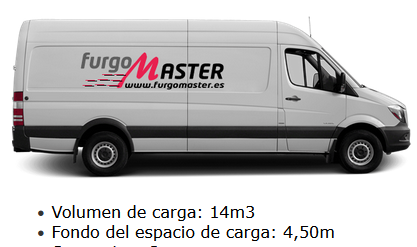
\includegraphics[scale=0.50]{imaxes/FurgonetaBase.png}
  \caption{\label{fig:FurgonetaBase}Ejemplo de la furgoneta base}
\end{figure}

\begin{figure}[H]
  \centering
  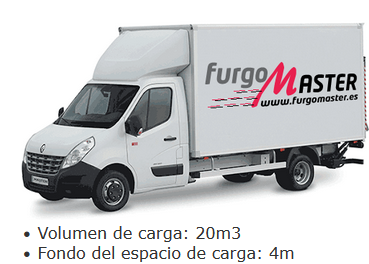
\includegraphics[scale=0.50]{imaxes/FurgonetaFrio.png}
  \caption{\label{fig:FurgonetaFrio}Ejemplo de la furgoneta para cargas en frio}
\end{figure}

\begin{figure}[H]
  \centering
  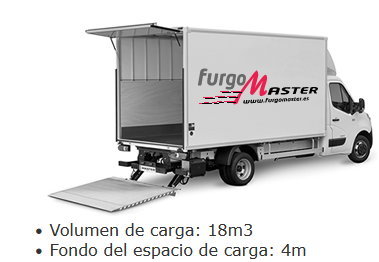
\includegraphics[scale=0.50]{imaxes/FurgonetaAnimales.png}
  \caption{\label{fig:FurgonetaAnimales}Ejemplo de la furgoneta para transportar animales}
\end{figure}

\begin{table}[H]
  \centering
  \resizebox{15,0cm}{!}{
    \begin{tabular}{|c|c|c|c|}
      \hline
      \multicolumn{4}{|c|}{\textbf{Lista de paquetes para asignar recursos para la Ruta A}} \\
      \hline \hline
      
      \multicolumn{1}{|p{1.0cm}|}{\centering \textsc{N\textordmasculine}} &\multicolumn{1}{|p{3.0cm}|}{\centering \textsc{Dimensión (cm)}} & \multicolumn{1}{|p{3.0cm}|}{\centering \textsc{Peso (kg)}} & \multicolumn{1}{|p{3.0cm}|}{\centering \textsc{Tipo de paquete}} \\
      \hline

      1 & \multicolumn{1}{|p{3.0cm}|}{\centering 30x30x30} & \multicolumn{1}{|p{3.0cm}|}{\centering 10} & \multicolumn{1}{|p{3.0cm}|}{\centering normal} \\
      \hline
      2 & \multicolumn{1}{|p{3.0cm}|}{\centering 200x100x40} & \multicolumn{1}{|p{3.0cm}|}{\centering 30} & \multicolumn{1}{|p{3.0cm}|}{\centering normal} \\
      \hline
      3 & \multicolumn{1}{|p{3.0cm}|}{\centering 100x50x40} & \multicolumn{1}{|p{3.0cm}|}{\centering 15} & \multicolumn{1}{|p{3.0cm}|}{\centering frio} \\
      \hline
    \end{tabular}
  }
	\caption{\label{tab:AsignarRecursoRutaA}Lista de paquetes asignados a la Ruta A}
\end{table}

\begin{table}[H]
  \centering
  \resizebox{15,0cm}{!}{
    \begin{tabular}{|c|c|c|c|}
      \hline
      \multicolumn{4}{|c|}{\textbf{Lista de paquetes para asignar recursos para la Ruta B}} \\
      \hline \hline
      
      \multicolumn{1}{|p{1.0cm}|}{\centering \textsc{N\textordmasculine}} &\multicolumn{1}{|p{3.0cm}|}{\centering \textsc{Dimensión (cm)}} & \multicolumn{1}{|p{3.0cm}|}{\centering \textsc{Peso (kg)}} & \multicolumn{1}{|p{3.0cm}|}{\centering \textsc{Tipo de paquete}} \\
      \hline

      1 & \multicolumn{1}{|p{3.0cm}|}{\centering 130x130x130} & \multicolumn{1}{|p{3.0cm}|}{\centering 10} & \multicolumn{1}{|p{3.0cm}|}{\centering normal} \\
      \hline
      
      2 & \multicolumn{1}{|p{3.0cm}|}{\centering 200x200x200} & \multicolumn{1}{|p{3.0cm}|}{\centering 20} & \multicolumn{1}{|p{3.0cm}|}{\centering animal} \\
      \hline
      
      3 & \multicolumn{1}{|p{3.0cm}|}{\centering 100x50x40} & \multicolumn{1}{|p{3.0cm}|}{\centering 15} & \multicolumn{1}{|p{3.0cm}|}{\centering frio} \\
      \hline
    \end{tabular}
  }
	\caption{\label{tab:AsignarRecursoRutaB}Lista de paquetes asignados a la Ruta B}
\end{table}

\begin{table}[H]
  \centering
  \resizebox{15,0cm}{!}{
    \begin{tabular}{|c|c|c|c|}
      \hline
      \multicolumn{4}{|c|}{\textbf{Lista de paquetes para asignar recursos para la Ruta C}} \\
      \hline \hline
      
      \multicolumn{1}{|p{1.0cm}|}{\centering \textsc{N\textordmasculine}} &\multicolumn{1}{|p{3.0cm}|}{\centering \textsc{Dimensión (cm)}} & \multicolumn{1}{|p{3.0cm}|}{\centering \textsc{Peso (kg)}} & \multicolumn{1}{|p{3.0cm}|}{\centering \textsc{Tipo de paquete}} \\
      \hline

      1 & \multicolumn{1}{|p{3.0cm}|}{\centering 130x130x130} & \multicolumn{1}{|p{3.0cm}|}{\centering 10} & \multicolumn{1}{|p{3.0cm}|}{\centering normal} \\
      \hline
      
      2 & \multicolumn{1}{|p{3.0cm}|}{\centering 200x200x200} & \multicolumn{1}{|p{3.0cm}|}{\centering 20} & \multicolumn{1}{|p{3.0cm}|}{\centering animal} \\
      \hline
      
      3 & \multicolumn{1}{|p{3.0cm}|}{\centering 100x50x40} & \multicolumn{1}{|p{3.0cm}|}{\centering 15} & \multicolumn{1}{|p{3.0cm}|}{\centering frio} \\
      \hline
    \end{tabular}
  }
	\caption{\label{tab:AsignarRecursoRutaC}Lista de paquetes asignados a la Ruta C}
\end{table}

Asignar recursos para las siguientes encenarios:
\begin{enumerate}
	\item  \textbf{Listado de carga para la Ruta A:} Asignar recursos para la entrega de la paquetería del listado de la Tabla \ref{tab:AsignarRecursoRutaA}.
	\item  \textbf{Listado de carga para la Ruta B:} Asignar recursos para la entrega de la paquetería del listado de la Tabla \ref{tab:AsignarRecursoRutaB}.
\end{enumerate}

\section{Fase de especificación}
\subsection{Justificación de la selección de la metodología}
Para este proyecto hemos decidido utilizar la metodología ``middle-out'' con la selección de la plantilla de configuración como se muestra en la Figura \ref{fig:PlantillaConfiguracion}, ya que esa plantilla nos permite buscar una mejor distribución de la carga dentro del vehículo asignado a la ruta. 

\begin{figure}[H]
  \centering
  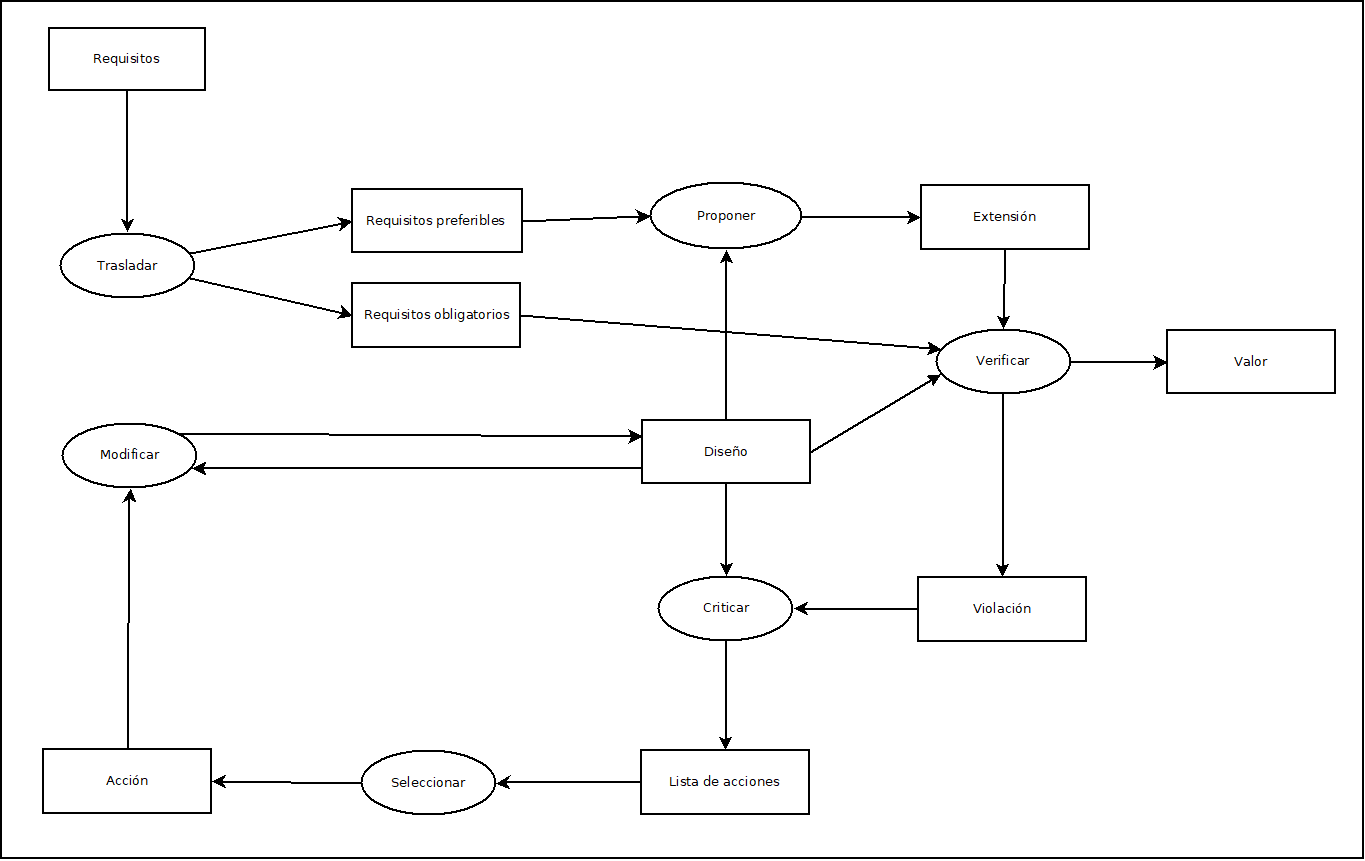
\includegraphics[scale=0.30]{imaxes/PlantillaConfiguracion.png}
  \caption{\label{fig:PlantillaConfiguracion}Ejemplo de la plantilla elegida}
\end{figure}

\subsection{Plantilla anotada}

La plantilla que mas se adapta a nuestro problema es la de configuración, como se muestra en la Figura \ref{fig:PlantillaConfiguracionComentada}.

\begin{figure}[H]
  \centering
  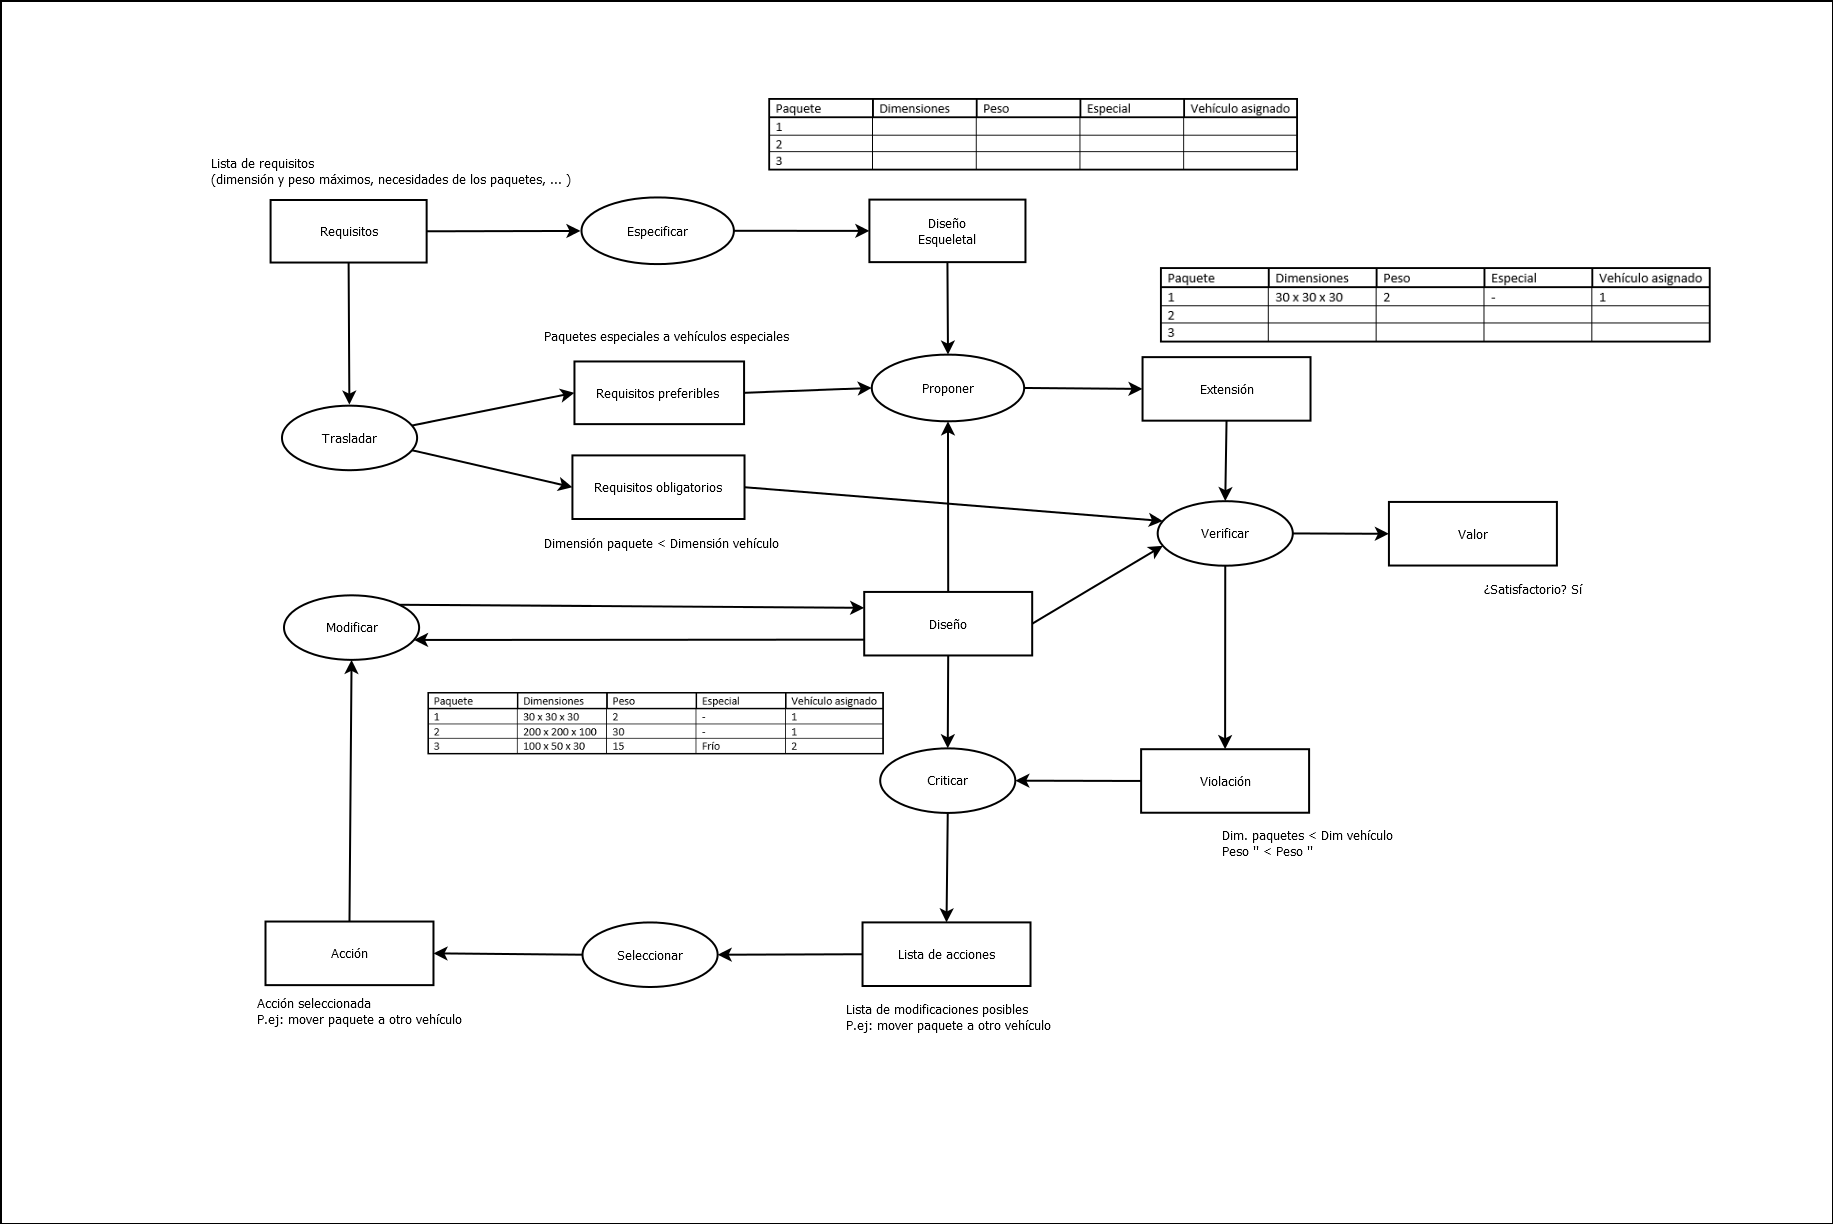
\includegraphics[scale=0.25]{imaxes/PlantillaConfiguracionComentada.png}
  \caption{\label{fig:PlantillaConfiguracionComentada}Ejemplo de la plantilla elegida con las anotaciones pertinentes}
\end{figure}

\newpage

\subsection{Esquema inicial del dominio}

\subsubsection{Plantilla}
La Figura \ref{fig:DiagramaInicialDominio} muestra el diagrama inicial del dominio.

\begin{figure}[H]
  \centering
  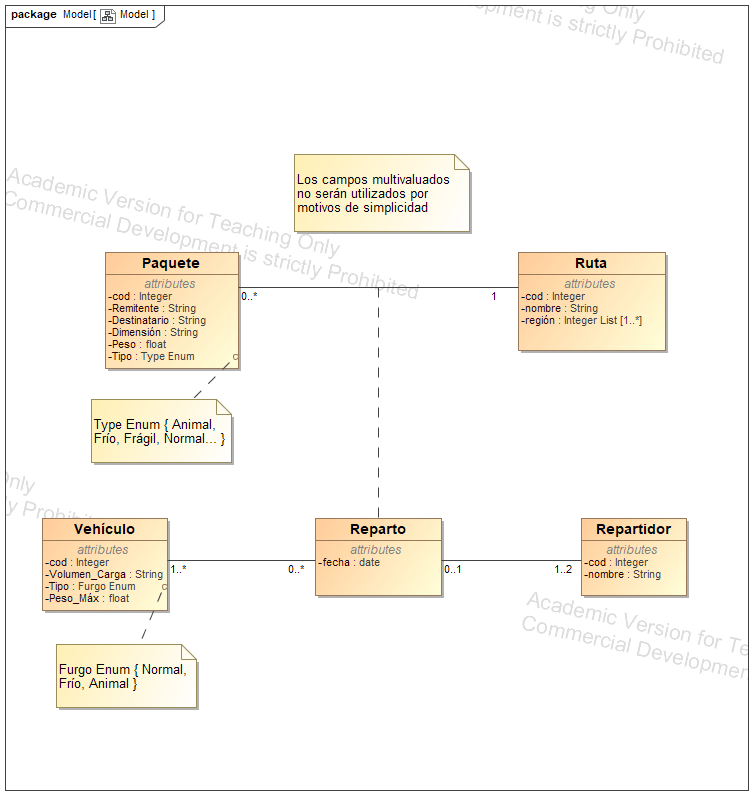
\includegraphics[scale=0.50]{imaxes/DiagramaInicialDominio.png}
  \caption{\label{fig:DiagramaInicialDominio}Diagrama inicial del dominio}
\end{figure}

\subsection{Estructura inferencial}

La Figura \ref{fig:EstructuraInferencial} muestra la estructura inferencial de la plantilla elegida.
\begin{figure}[H]
  \centering
  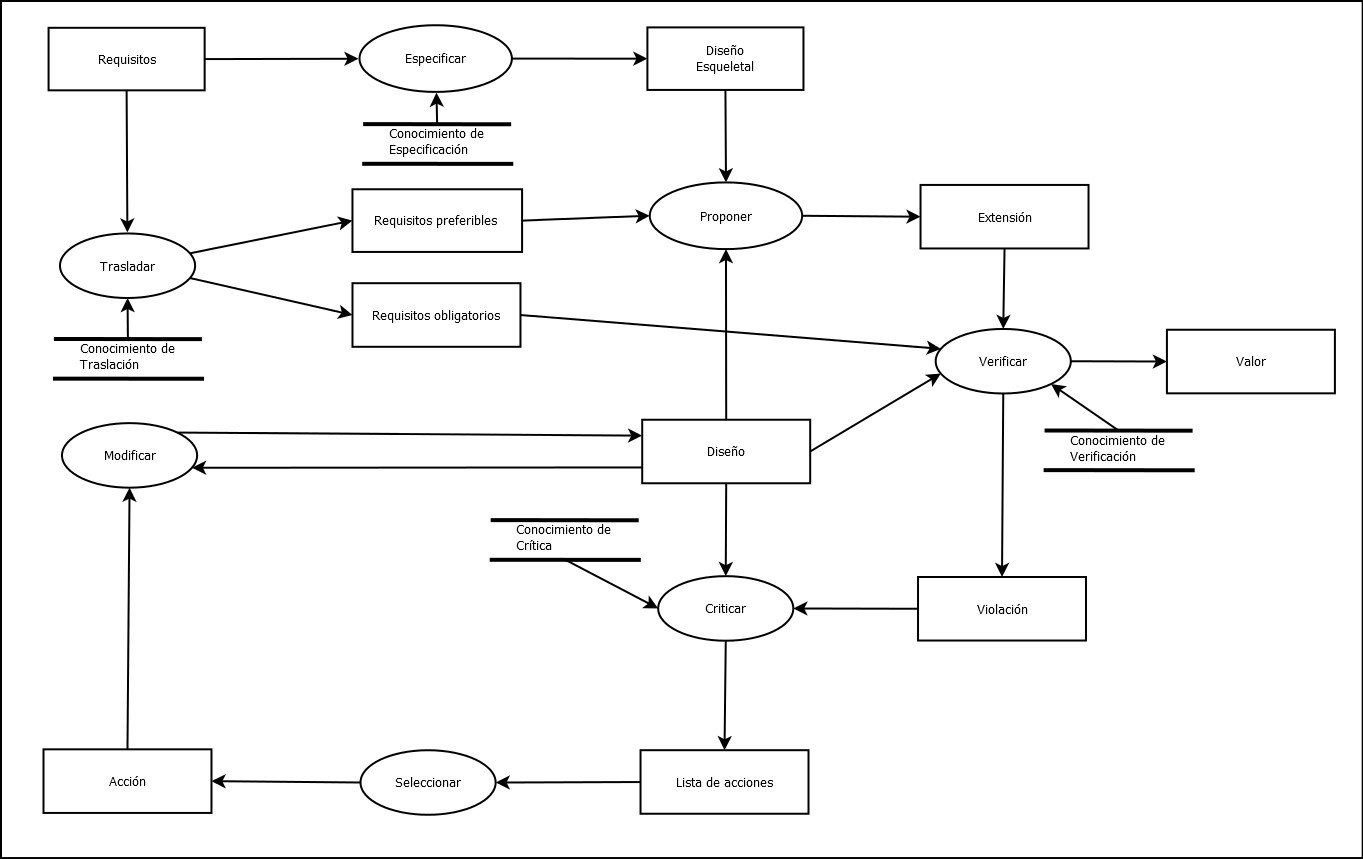
\includegraphics[scale=0.30]{imaxes/PlantillaInferencial.png}
  \caption{\label{fig:EstructuraInferencial}Estructura inferencial de la plantilla elegida}
\end{figure}

\subsubsection{Mapeado}

Relacción entre los roles de las inferencias de la plantilla con los conceptos de nuestro problema.

La Figura \ref{fig:TrasladarPreferibles} muestra el mapeo de la inferencia \textbf{\textit{Trasladar}} a \textit{Requisitos preferibles}.

\begin{figure}[H]
  \centering
  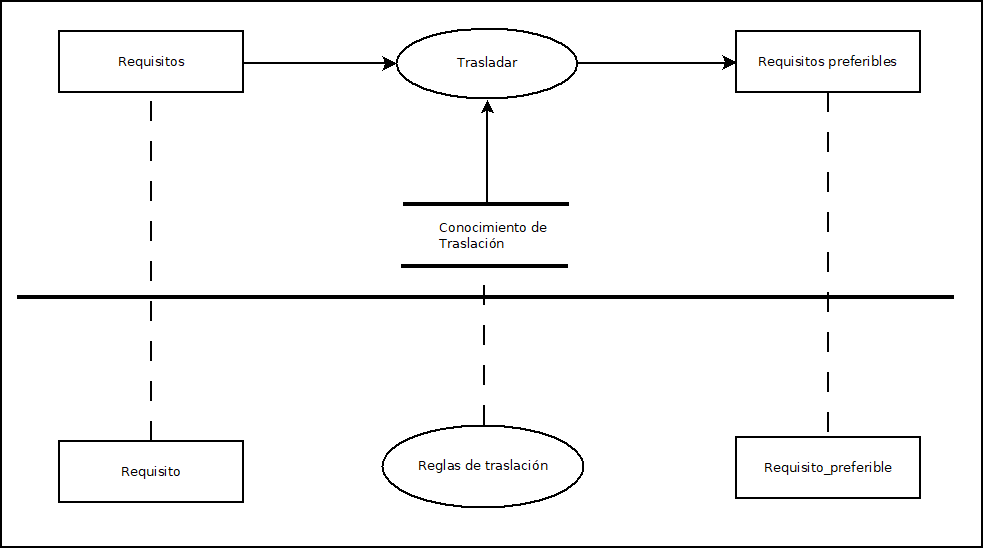
\includegraphics[scale=0.35]{imaxes/TrasladarPreferibles.png}
  \caption{\label{fig:TrasladarPreferibles}Mapeado de \textit{Trasladar} a \textit{Requisitos preferibles}.}
\end{figure}

La Figura \ref{fig:TrasladarObligatorios} muestra el mapeo de la inferencia \textbf{\textit{Trasladar}} a \textit{Requisitos obligatorios}.

\begin{figure}[H]
  \centering
  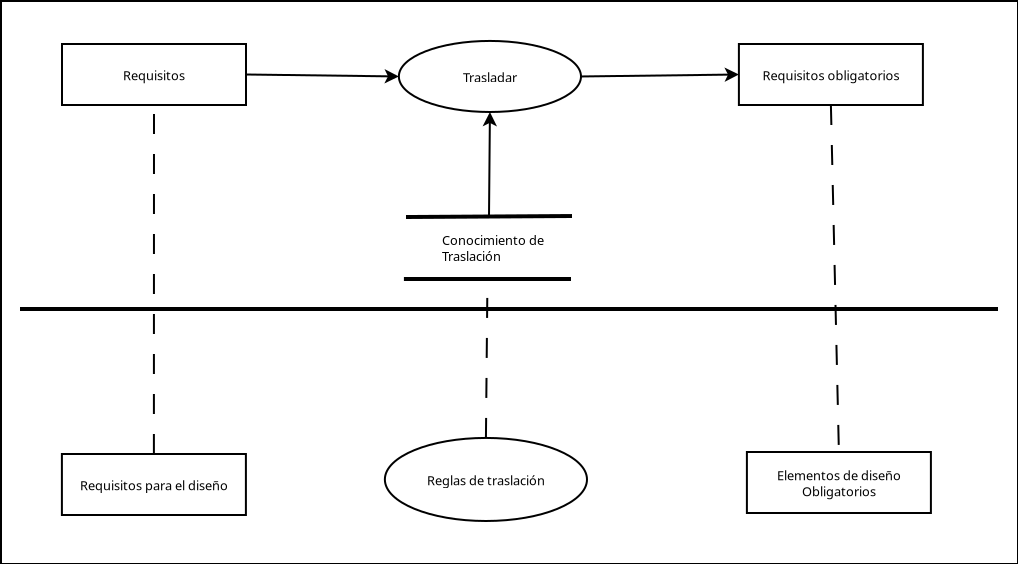
\includegraphics[scale=0.35]{imaxes/TrasladarObligatorios.png}
  \caption{\label{fig:TrasladarObligatorios}Mapeado de \textit{Trasladar} a \textit{Requisitos obligatorios}.}
\end{figure}

La Figura \ref{fig:PreferiblesProponerExtension} muestra el mapeo de la inferencia \textbf{Proponer} elementos preferibles.

\begin{figure}[H]
  \centering
  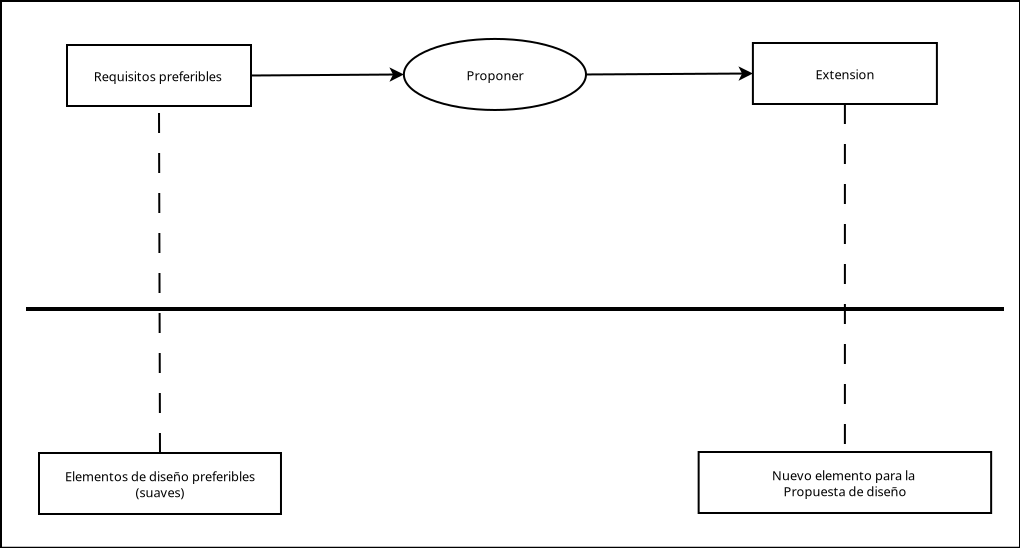
\includegraphics[scale=0.35]{imaxes/PreferiblesProponerExtension.png}
  \caption{\label{fig:PreferiblesProponerExtension}Mapeado de \textit{proponer} elementos preferibles.}
\end{figure}

La Figura \ref{fig:DisenoProponerExtension} muestra el mapeo de la inferencia \textbf{Proponer} diseño actual o modificado.

\begin{figure}[H]
  \centering
  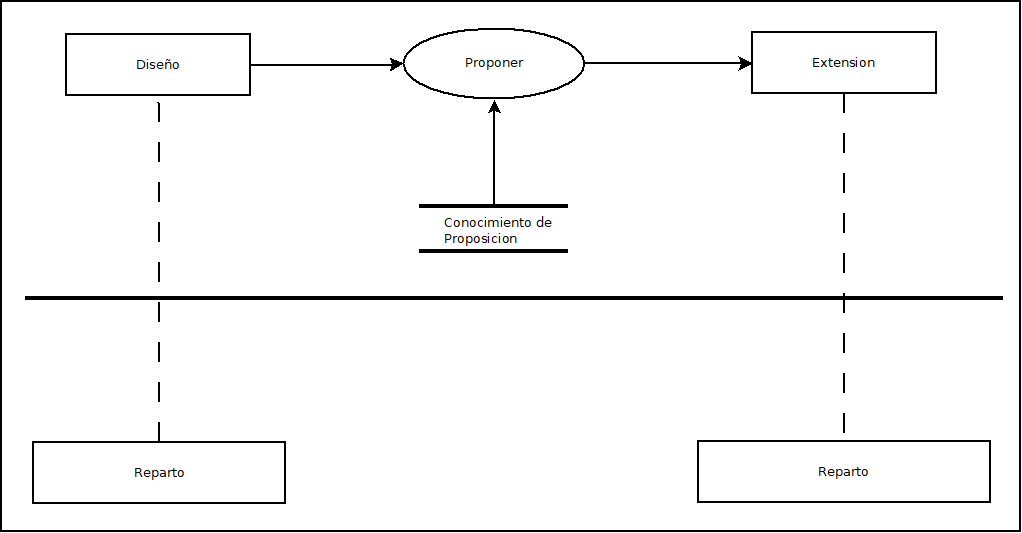
\includegraphics[scale=0.35]{imaxes/DisenoProponerExtension.png}
  \caption{\label{fig:DisenoProponerExtension}Mapeado de \textit{Proponer} diseño actual o modificado.}
\end{figure}

La Figura \ref{fig:DisenoVerificarValor} muestra el mapeo de la inferencia \textbf{Verificar} diseño actual o modificado.

\begin{figure}[H]
  \centering
  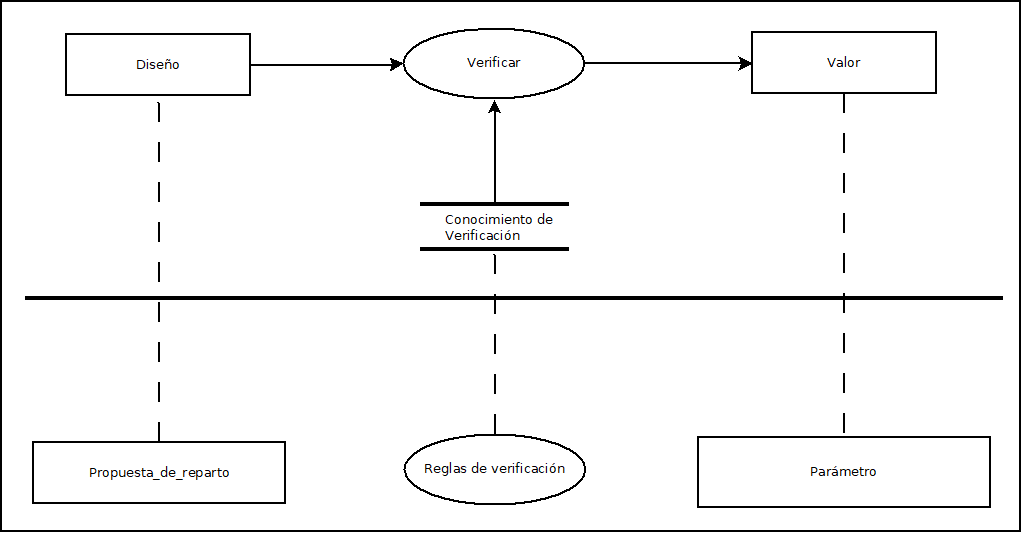
\includegraphics[scale=0.35]{imaxes/DisenoVerificarValor.png}
  \caption{\label{fig:DisenoVerificarValor}Mapeado de \textit{Verificar} diseño actual o modificado.}
\end{figure}

La Figura \ref{fig:RequisitosObligatoriosVerificarValor} muestra el mapeo de la inferencia \textbf{Verificar} requisitos obligatorios de diseño.

\begin{figure}[H]
  \centering
  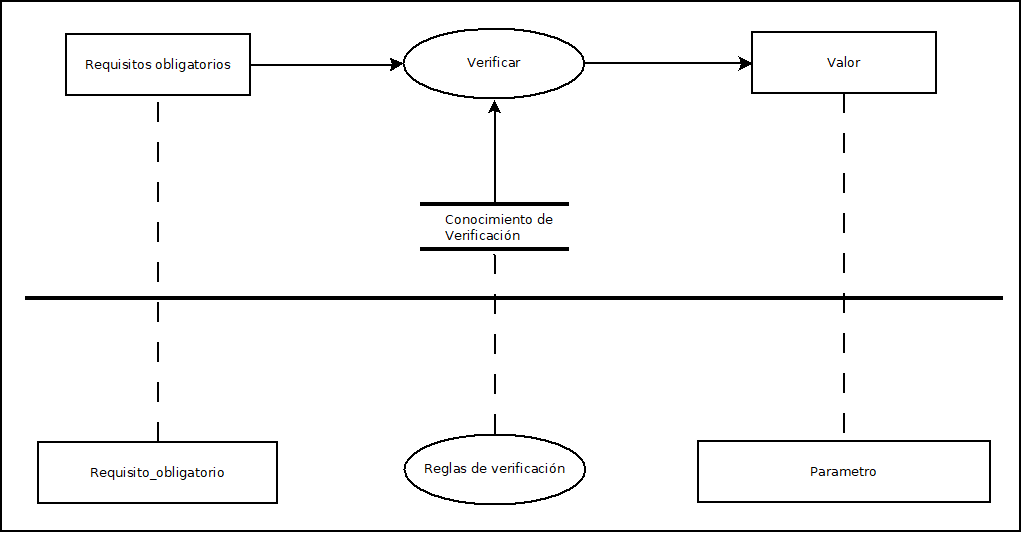
\includegraphics[scale=0.35]{imaxes/RequisitosObligatoriosVerificarValor.png}
  \caption{\label{fig:RequisitosObligatoriosVerificarValor}Mapeado de \textit{Verificar} diseño elemental.}
\end{figure}

La Figura \ref{fig:DisenoVerificarViolacion} muestra el mapeo de la inferencia \textbf{Verificar} la violación de un elemento de diseño.

\begin{figure}[H]
  \centering
  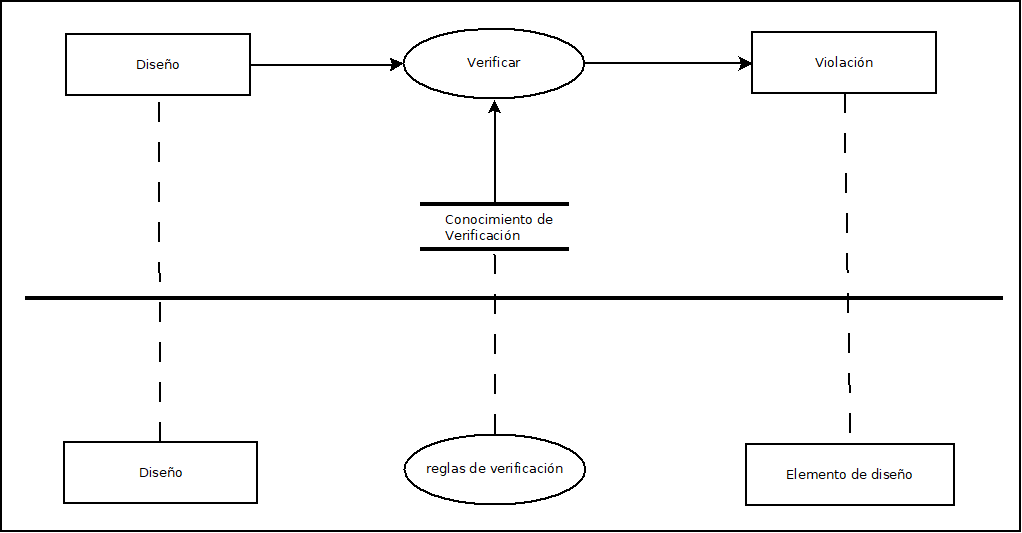
\includegraphics[scale=0.35]{imaxes/DisenoVerificarViolacion.png}
  \caption{\label{fig:DisenoVerificarViolacion}Mapeado de \textit{Verificar} la violación de un elemento de diseño.}
\end{figure}

La Figura \ref{fig:ExtensionVerificarViolacion} muestra el mapeo de la inferencia \textbf{Verificar} la violación de un nuevo elemento de diseño.

\begin{figure}[H]
  \centering
  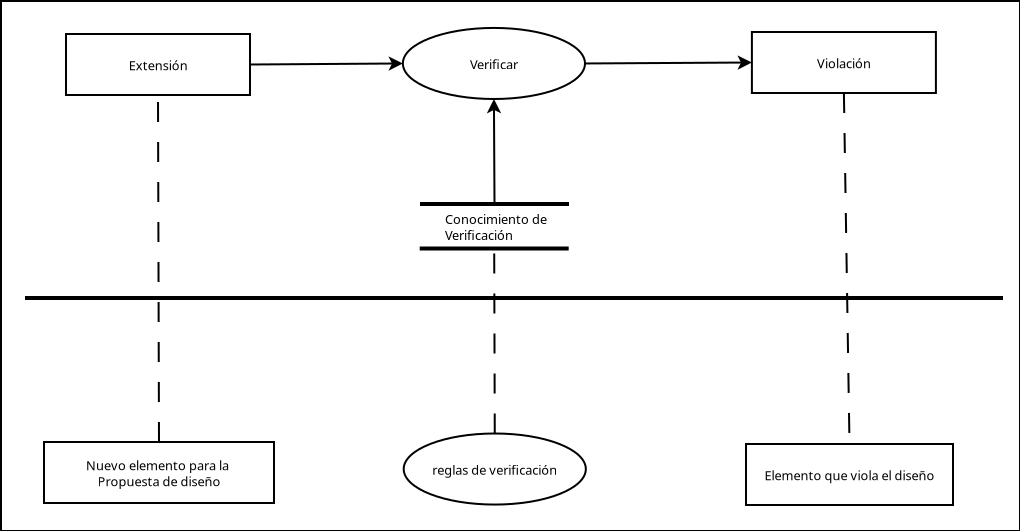
\includegraphics[scale=0.35]{imaxes/ExtensionVerificarViolacion.png}
  \caption{\label{fig:ExtensionVerificarViolacion}Mapeado de \textit{Verificar} la violación de un nuevo elemento de diseño.}
\end{figure}

La Figura \ref{fig:RequisitosObligatoriosVerificarViolacion} muestra el mapeo de la inferencia \textbf{Verificar} la violación de requisitos obligatorios.

\begin{figure}[H]
  \centering
  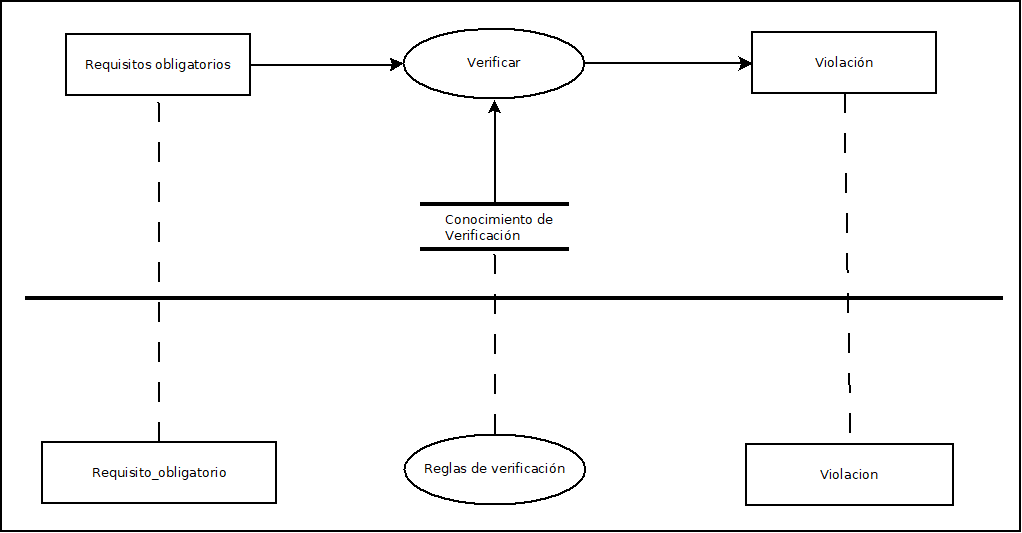
\includegraphics[scale=0.35]{imaxes/RequisitosObligatoriosVerificarViolacion.png}
  \caption{\label{fig:RequisitosObligatoriosVerificarViolacion}Mapeado de \textit{Verificar} la violación de requisitos obligatorios.}
\end{figure}

La Figura \ref{fig:DisenoCriticarListaAciones} muestra el mapeo de la inferencia \textbf{Criticar} el diseño.

\begin{figure}[H]
  \centering
  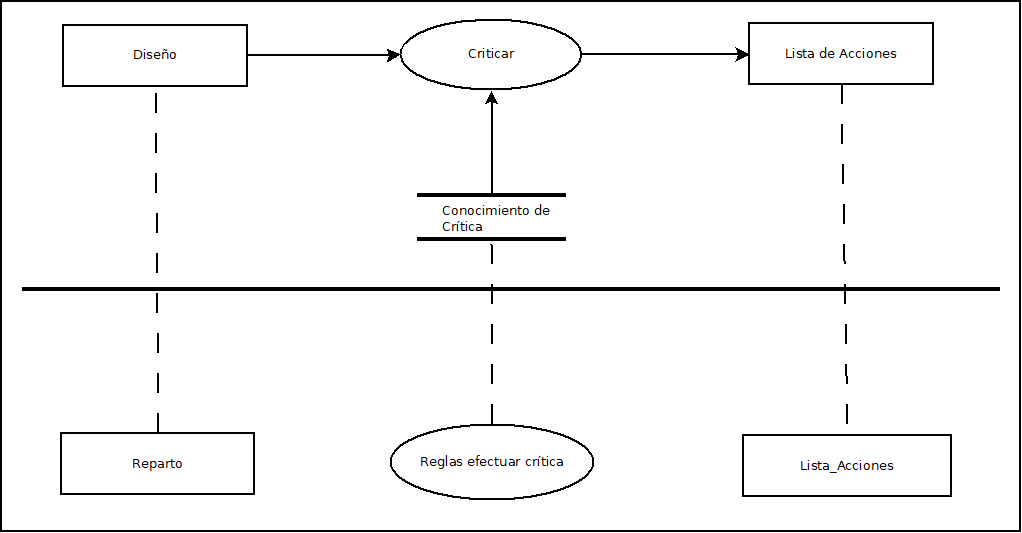
\includegraphics[scale=0.35]{imaxes/DisenoCriticarListaAciones.png}
  \caption{\label{fig:DisenoCriticarListaAciones}Mapeado de \textit{Criticar} el diseño.}
\end{figure}

La Figura \ref{fig:ViolacionCriticarListaAciones} muestra el mapeo de la inferencia \textbf{Criticar} la violación del diseño.

\begin{figure}[H]
  \centering
  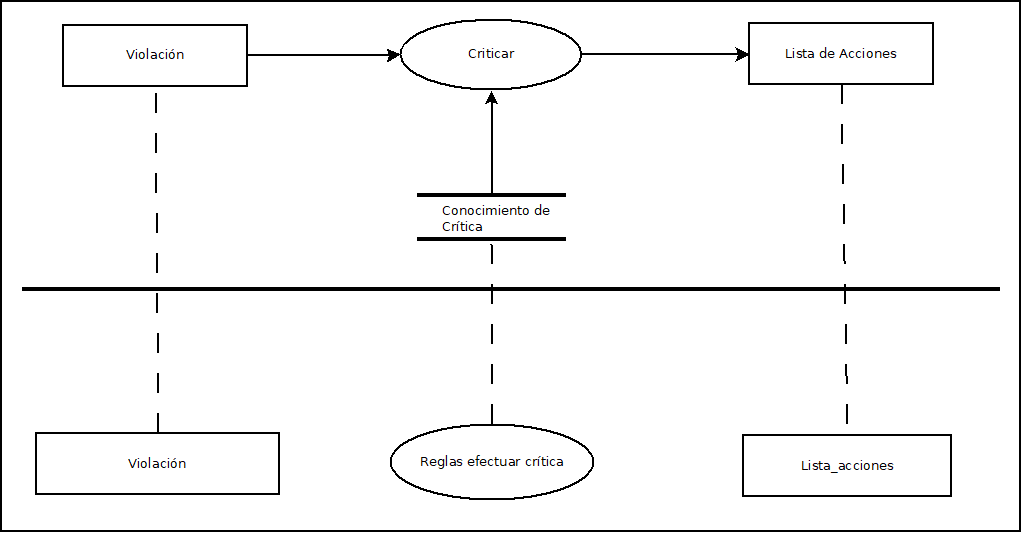
\includegraphics[scale=0.35]{imaxes/ViolacionCriticarListaAciones.png}
  \caption{\label{fig:ViolacionCriticarListaAciones}Mapeado de \textit{Criticar} la violación del diseño.}
\end{figure}

La Figura \ref{fig:ListaAccionesSeleccionarAccion} muestra el mapeo de la inferencia \textbf{Seleccionar} acción de la lista de acciones.

\begin{figure}[H]
  \centering
  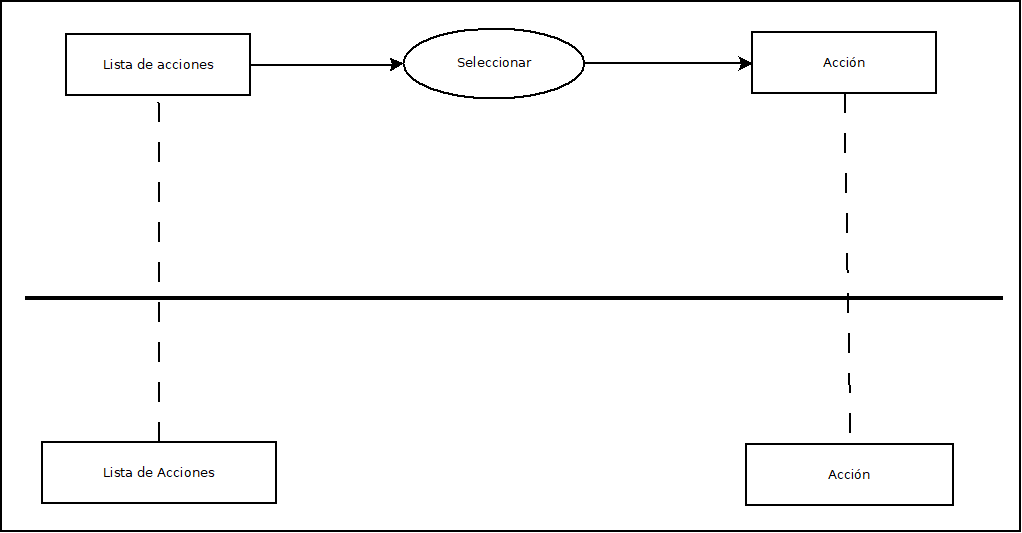
\includegraphics[scale=0.35]{imaxes/ListaAccionesSeleccionarAccion.png}
  \caption{\label{fig:ListaAccionesSeleccionarAccion}Mapeado de \textit{Seleccionar} accion de la lista de acciones.}
\end{figure}

La Figura \ref{fig:AccionModificaDiseno} muestra el mapeo de la inferencia \textbf{Modificar} diseño.

\begin{figure}[H]
  \centering
  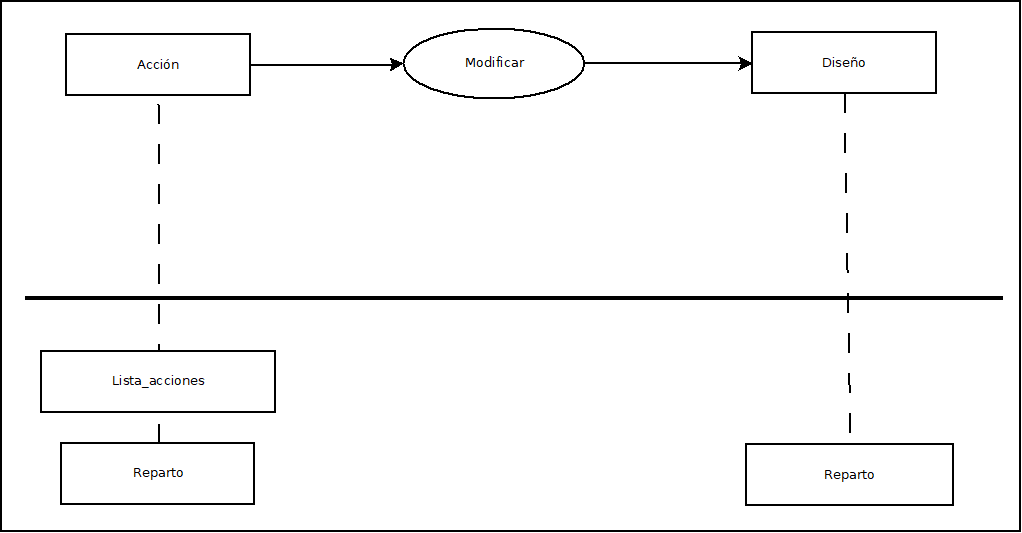
\includegraphics[scale=0.35]{imaxes/AccionModificaDiseno.png}
  \caption{\label{fig:AccionModificaDiseno}Mapeado de \textit{Modificar} diseño.}
\end{figure}

La Figura \ref{fig:DisenoModificarDiseno} muestra el mapeo de la inferencia \textbf{Modificar} diseño desde diseño.

\begin{figure}[H]
  \centering
  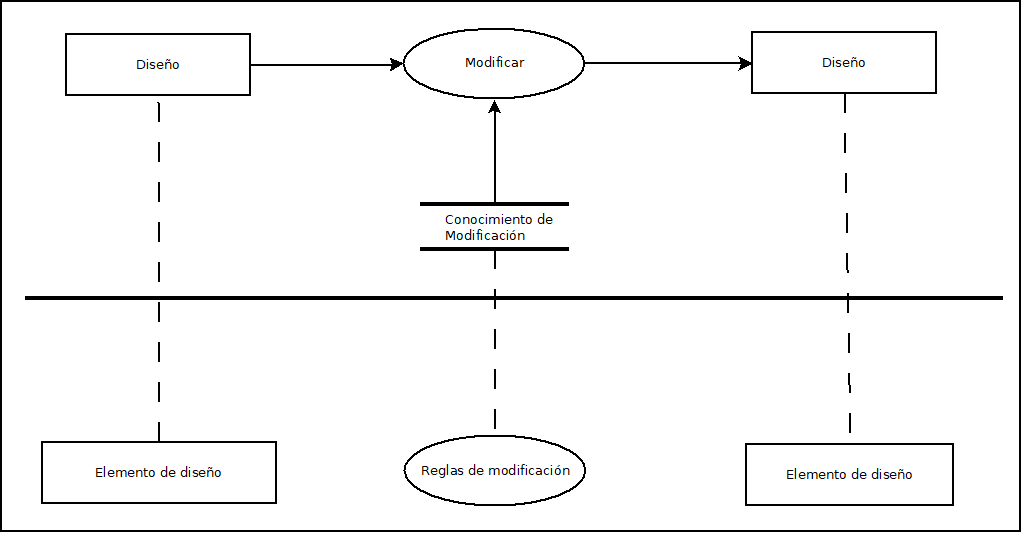
\includegraphics[scale=0.35]{imaxes/DisenoModificarDiseno.png}
  \caption{\label{fig:DisenoModificarDiseno}Mapeado de \textit{Modificar} diseño desde diseño.}
\end{figure}


\section{Especificación y método de la tarea}

\subsection{Especificación}

\begin{lstlisting}[language=C,caption=\textbf{Especificación}]
  TASK configuracion-diseño;
    ROLES:
      INPUT: Requisitos: "requisitos para el diseño";
      OUTPUT: Diseño: "el diseño resultante";
  END TASK configuracion-diseño;
\end{lstlisting}

\newpage
\subsection{Método de la Tarea}

\begin{lstlisting}[language=C,caption=\textbf{Método de la tarea}]
  TASK-METHOD proponer-y-revisar;
    REALIZES: configuracion-diseño;
    DECOMPOSITION:
      INFERENCES: Trasladar, Especificar, Proponer, Verificar, Criticar, Seleccionar, Modificar;
    ROLES:
      INTERMEDIATE:
        Requisitos-preferibles: "requisitos que se utilizarán como preferencias (suaves)";
        Requisitos-obligatorios: "requisitos que son restricciones obligatorias (estrictas)";
        Diseño-Esqueletal: "conjunto de elementos de diseño";
        Extensión: "un único valor nuevo para un elemento de diseño";
        Violación: "restricción violada por el diseño actual";
        Valor: "booleano que indica el resultado de la verificación";
        Lista-de-acciones: "lista ordenada de posibles acciones de reparación (fijación)";
        Acción: "una sola acción de reparación";
    CONTROL-STRUCTURE:
      operacionalizar(Requisitos -> Requisitos-preferibles + Requisitos-obligatorios);
      especificar(Requisitos -> Diseño-Esqueletal);
      WHILE NEW-SOLUTION proponer(Diseño-Esqueletal + Diseño + Requisitos-preferibles -> Extensión) DO
        Diseño := Extensión ADD Diseño;
        verificar(Diseño + Requisitos-obligatorios -> Valor + Violación);
        IF Valor == false
        THEN
          criticar(Violación + Diseño -> Lista-de-acciones);
          REPEAT
            seleccionar(Lista-de-acciones -> Acción);
            modificar(Diseño + Acción -> Diseño);
            verificar(Diseño + Requisitos-obligatorios -> Valor + Violación);
          UNTIL Valor == true;
          END REPEAT
        END IF
      END WHILE
  END TASK-METHOD proponer-y-revisar;
\end{lstlisting}

\subsection{Base de conocimiento}

\begin{lstlisting}[language=C,caption=\textbf{Regla\_de\_Traslación}]
  EXPRESSIONS:
    Requisito == Tipo_Requisito_preferible
  RESULTA_EN:
    Requisito_preferible
  END KNOWLEDGE-BASE Regla-translación;
    
  EXPRESSIONS:
    Requisito == Tipo_Requisito_obrigatorio
  RESULTA_EN:
    Requisito_obligatorio
  END KNOWLEDGE-BASE Regla_de_translación;
\end{lstlisting}


\begin{lstlisting}[language=C,caption=\textbf{Regla\_de\_Verificación}]
  EXPRESSIONS:
   (Reparto.Fecha == fecha_actual AND Reparto.Repartidor.Cod == 1 AND Reparto.Vehiculo.Cod == 1 AND Reparto.pesototal <= Vehiculo.peso_max AND Parametro.valor == false AND Requisitos_obligatorios == Peso) == true
  RESULTA EN:
   Reparto.violacion = V_peso 
  END KNOWLEDGE-BASE Regla_de_Verificación;
  
  EXPRESSIONS:
   (reparto.fecha == fecha_actual AND reparto.repartidor.cod == 1 AND reparto.vehiculo.cod == 1 AND reparto.volumentotal <= vehiculo.volumen_carga AND parametro.valor == false AND requisitos_obligatorios == Volumen) == true
  RESULTA EN:
   Reparto.violacion = V_Volumen 
  END KNOWLEDGE-BASE Regla_de_Verificación;
  
  EXPRESSIONS:
   (reparto.fecha == fecha_actual AND reparto.repartidor.cod == 1 AND reparto.vehiculo.cod == 1 AND reparto.volumentotal <= vehiculo.volumen_carga AND parametro.valor == false AND requisitos_obligatorios == Volumen) == false
  RESULTA EN:
   Reparto.violacion = V_noViola 
  END KNOWLEDGE-BASE Regla_de_Verificación;
\end{lstlisting}

\newpage    

\begin{lstlisting}[language=C,caption=\textbf{Regla\_de\_critica}]
  EXPRESSIONS:
    (reparto.fecha == fecha_actual AND reparto.repartidor.cod == 1 AND reparto.vehiculo.cod == 1 AND (Violación == V_peso OR Violación == V_volumen)) == true 
  CONDICIONA-A:
    Reparto.Lista_Acciones = Accion_Borrar
  END KNOWLEDGE-BASE regla_de_critica;
  
  EXPRESSIONS:
    (reparto.fecha == fecha_actual AND reparto.repartidor.cod == 1 AND reparto.vehiculo.cod == 1 AND (Violación == V_peso OR Violación == V_volumen)) == false 
  CONDICIONA-A:
    Reparto.Lista_Acciones = No_Hacer_Nada
  END KNOWLEDGE-BASE regla_de_critica;
\end{lstlisting}
      
\newpage

\subsection{Esquema completo del dominio}
Ahora que ya tenemos avanzado en el desarrollo de nuestro sistema inteligente, podemos ver como ha ido aumentando el esquema del dominio, tanto en entidades como relaciones, que ahora contienen las relaciones lógicas con el conocimiento del dominio. En la Figura \ref{fig:DominioCompleto} muestra el esquema de dominio final.

\begin{figure}[H]
  \centering
  %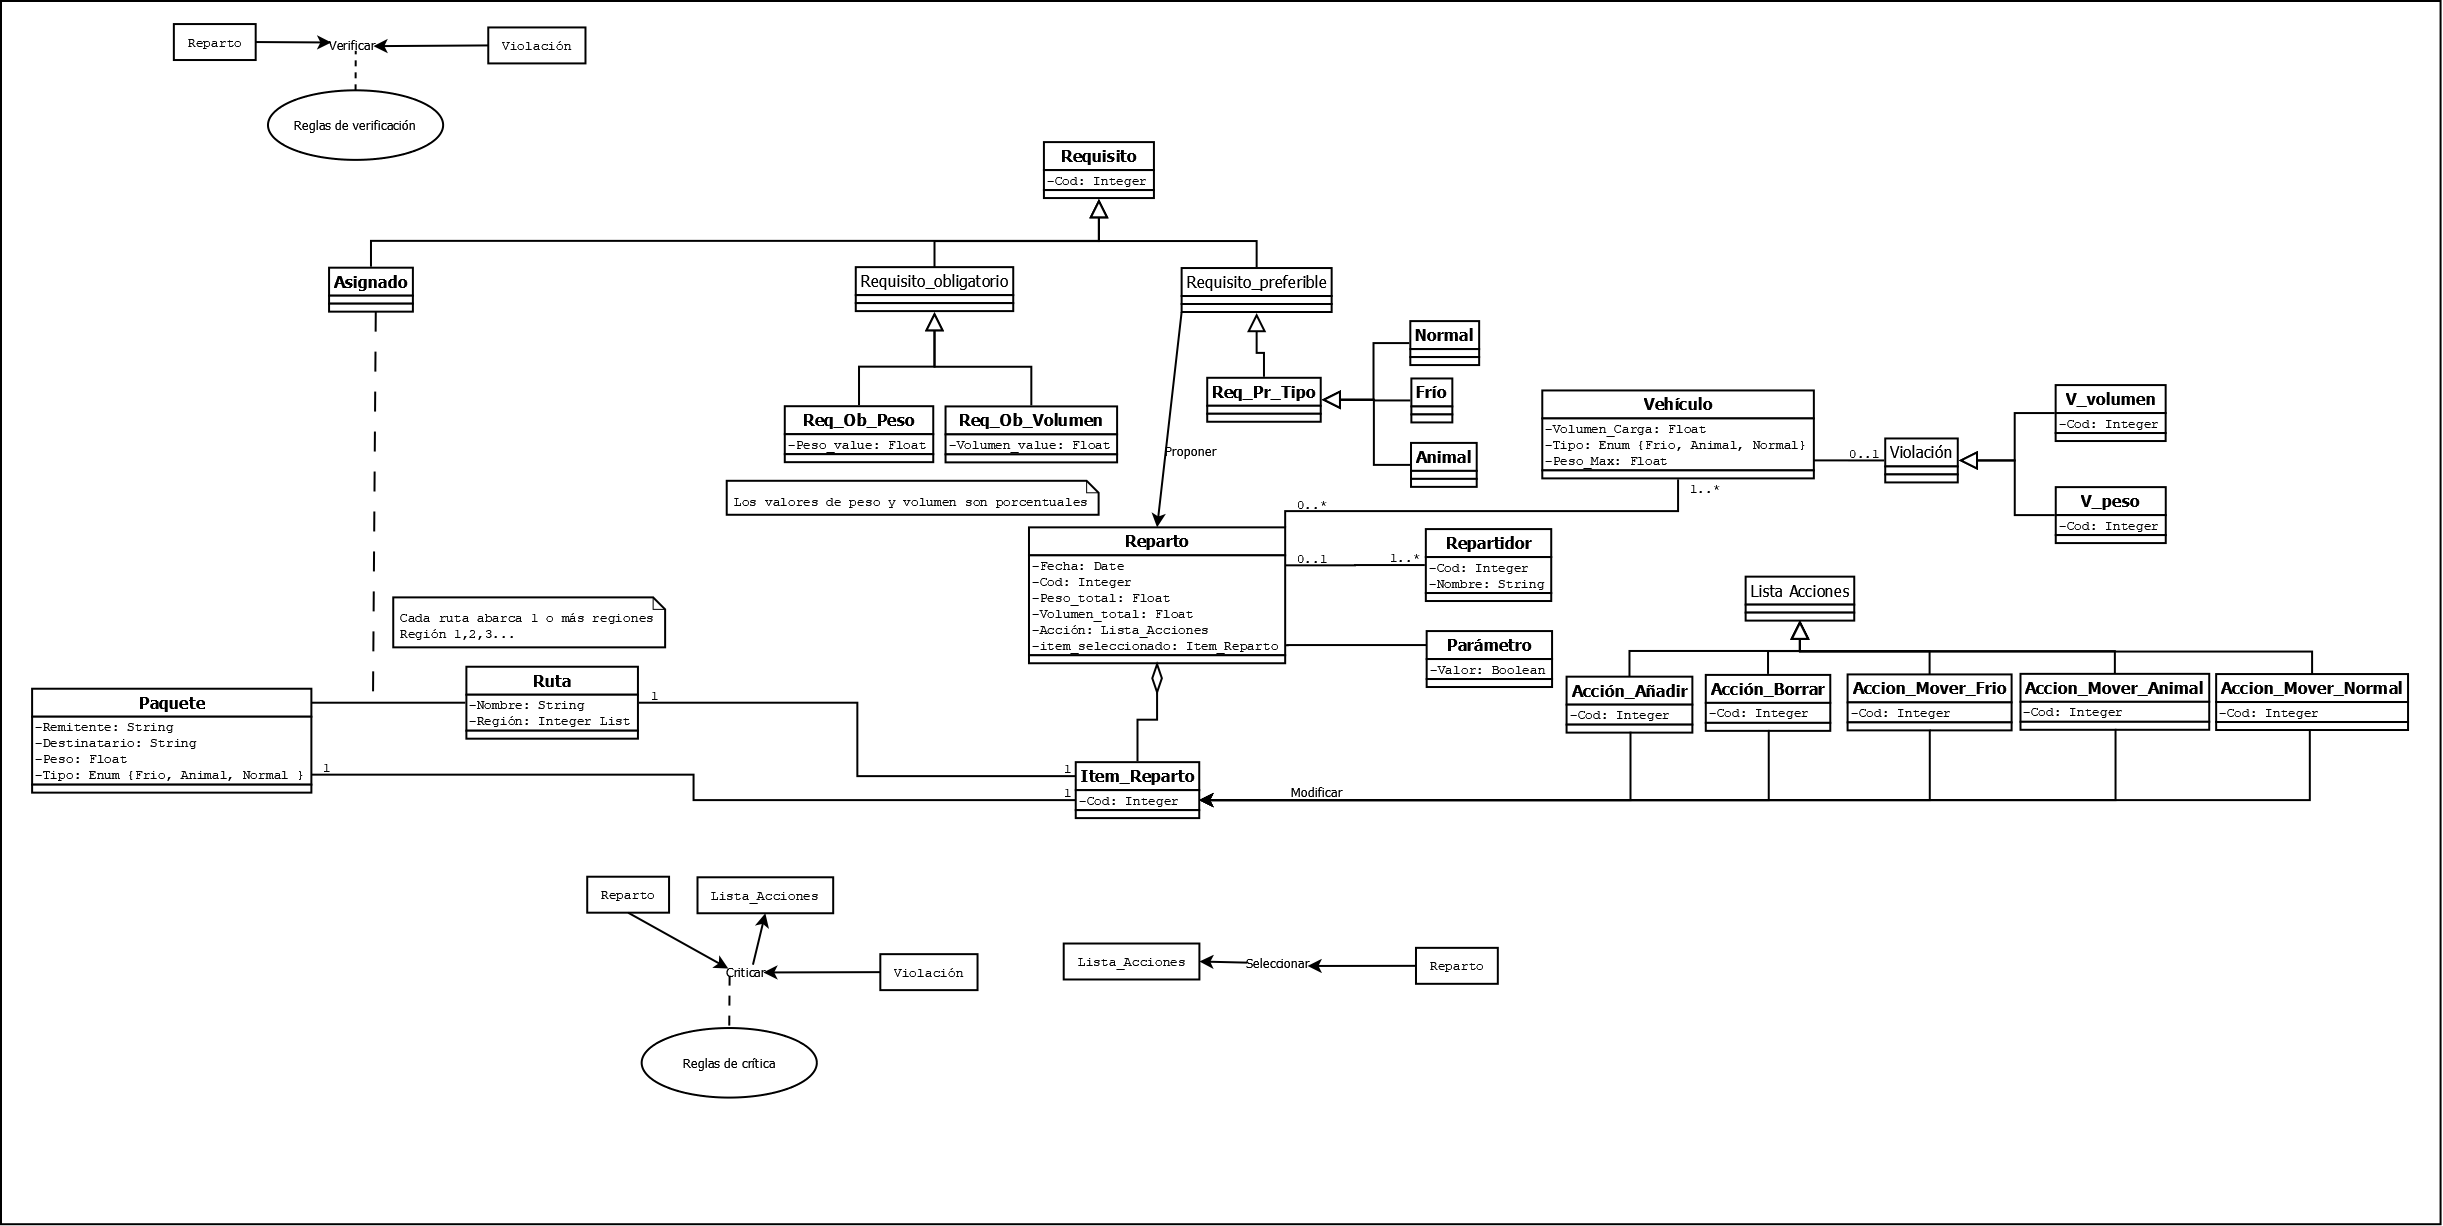
\includegraphics[scale=0.25,angle=90]{imaxes/Diagrama_Dominio_Completo.png}
  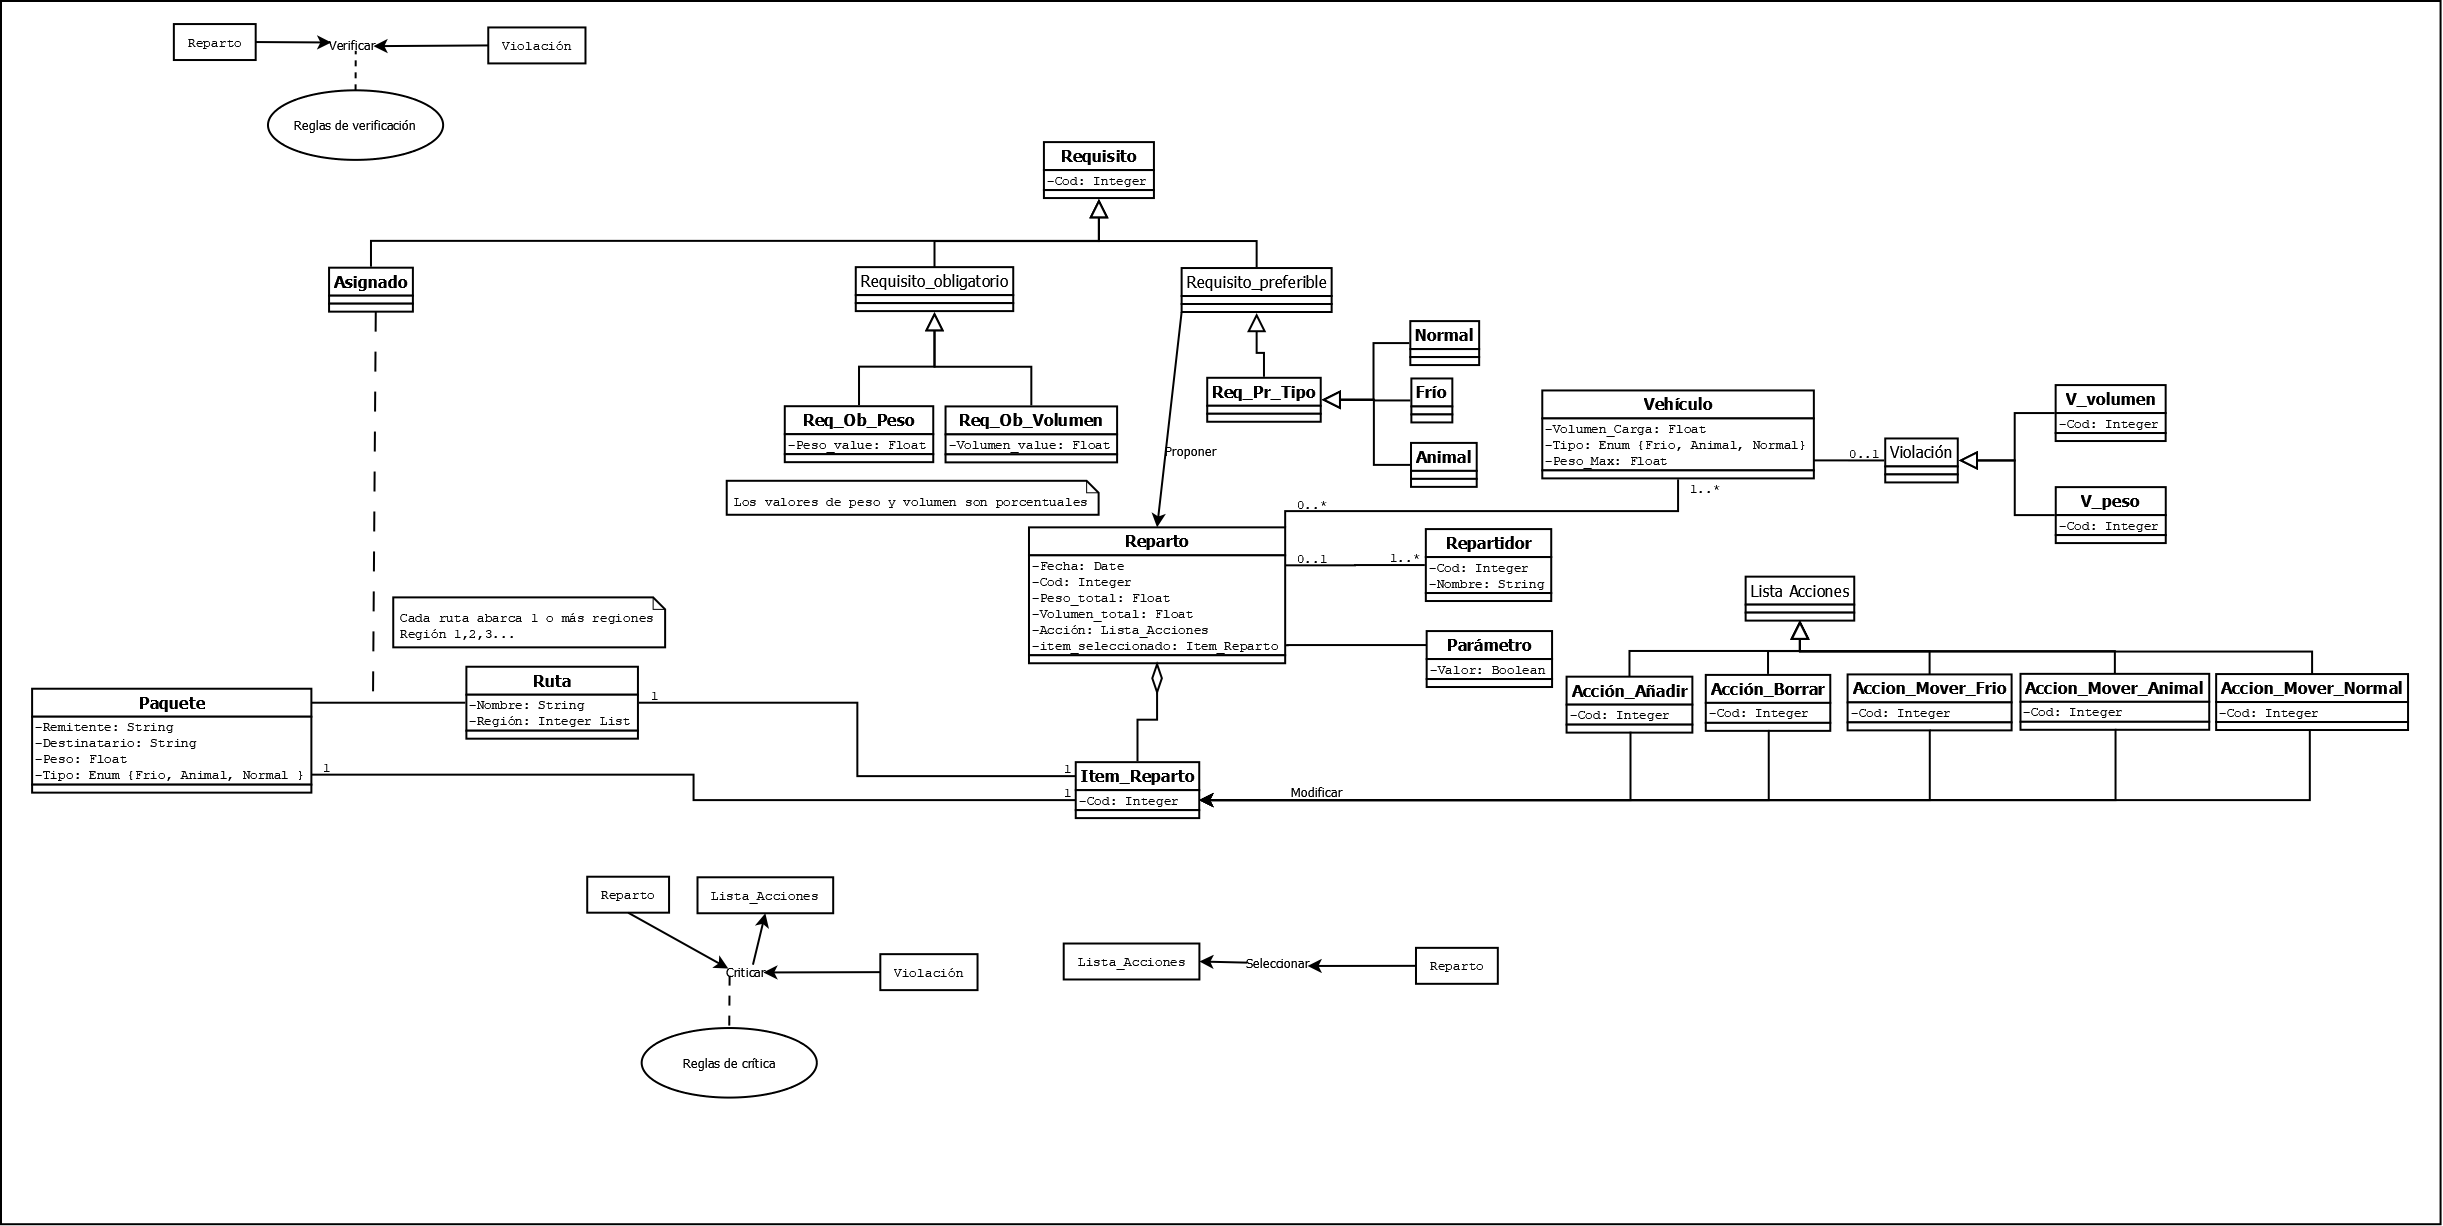
\includegraphics[scale=0.20, angle=90]{imaxes/Diagrama_Dominio_Completo.png}
  \caption{\label{fig:DominioCompleto}Esquema completo del dominio}
\end{figure}

%%%%%%%%%%%%%%%%%%%%%%%%%%%%%%%%%%%%%%%%%%%%%%%%%%%%%%%%%%%%%%%%%%%%%%%%
% Plantilla TFG/TFM
% Universidad de A Coruña. Facultad de Informática
% Realizado por: Welton Vieira dos Santos
% Modificado: Welton Vieira dos Santos
% Contacto: welton.dossantos@udc.es
%%%%%%%%%%%%%%%%%%%%%%%%%%%%%%%%%%%%%%%%%%%%%%%%%%%%%%%%%%%%%%%%%%%%%%%%


\chapter{Modelo de Comunicación}

\section{Plan de comunicación de comunicación general}
En este caso, la comunicación que se realiza es simplemente entre nuestro sistema y otros agentes para obtener dados referentes al mercado.

\subsection{Diagrama de diálogo}

  \begin{figure}[H]
    \centering
    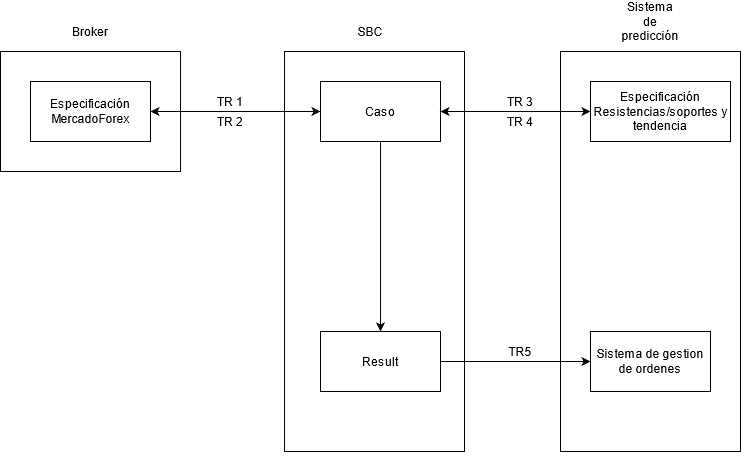
\includegraphics[scale=0.23]{imaxes/Comunicaciones.png}
    \caption{\label{fig:Comunicaciones}Diagrama de dialogo}
  \end{figure}
  
\subsection{Informacion de control de las transacciones}

  \begin{figure}[H]
    \centering
    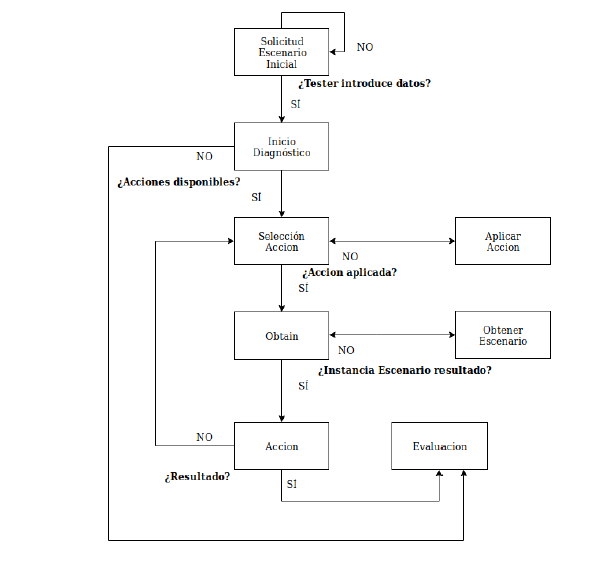
\includegraphics[scale=0.50]{imaxes/ControlTransacciones.png}
    \caption{\label{fig:ControlTransacciones}Diagrama de estados del sistema base de transacciones}
  \end{figure}
  
\subsection{Descripción de las transacciones}

\begin{table}[H]
  \scriptsize
  \begin{tabularx}{\textwidth}{|l|X|} \hline
    & \textbf{Formulario CM-1: Especificación de transacciones - TR1} \\
    \hline\hline
    {Nombre de la transacción} & Solicitar datos iniciales\\
    \hline  
    \textsc{Objecto de informacion} & \textsc{El SBC solicita información sobre la paquetería al sistema de gestión de MRW}\\ 
    \hline
    \textsc{Agentes involucrados} & \textsc{Emisor: SBC, Receptor: Sistema de gestión de MRW}\\ 
    \hline
    \textsc{Plan de comunicación} & \textsc{Especificado en las Figura \ref{fig:Comunicaciones} }\\ 
    \hline
    \textsc{Restricciones} & \textsc{El sistema de gestión debe estar en funcionamiento para realizar la solicitud}\\ 
    \hline
    \textsc{Especificación del intercambio} & \textsc{Tipo ASK}\\ 
    \hline
  \end{tabularx}
  \caption{\label{tab:TR1}Formulario CM-1 para TR-1}
\end{table}
  

\begin{table}[H]
  \scriptsize
  \begin{tabularx}{\textwidth}{|l|X|} \hline
    & \textbf{Formulario CM-1: Especificación de transacciones - TR2} \\
    \hline\hline
    {Nombre de la transacción} & Recibir datos iniciales\\
    \hline  
    \textsc{Objecto de informacion} & \textsc{El sistema de gestión envía la información necesaria sobre paquetería al SBC}\\ 
    \hline
    \textsc{Agentes involucrados} & \textsc{Emisor: Sistema de gestión de MRW, Receptor: SBC}\\ 
    \hline
    \textsc{Plan de comunicación} & \textsc{Especificado en la Figura \ref{fig:Comunicaciones} }\\ 
    \hline
    \textsc{Restricciones} & \textsc{El SBC debe estar listo para su uso}\\ 
    \hline
    \textsc{Especificación del intercambio} & \textsc{Tipo REPLY}\\ 
    \hline
  \end{tabularx}
  \caption{\label{tab:TR2}Formulario CM-1 para TR-2}
\end{table}


\begin{table}[H]
  \scriptsize
  \begin{tabularx}{\textwidth}{|l|X|} \hline
    & \textbf{Formulario CM-1: Especificación de transacciones - TR3} \\
    \hline\hline
    {Nombre de la transacción} & Solicitud de la Revisión y Validación\\
    \hline  
    \textsc{Objecto de informacion} & \textsc{El SBC solicita la confirmación de la distribución por parte del equipo directivo}\\ 
    \hline
    \textsc{Agentes involucrados} & \textsc{Emisor: SBC, Receptor: Equipo Directivo.}\\ 
    \hline
    \textsc{Plan de comunicación} & \textsc{Especificado en la Figura \ref{fig:Comunicaciones} }\\ 
    \hline
    \textsc{Restricciones} & \textsc{El equipo directivo debe estar disponible para realizar la confirmación}\\ 
    \hline
    \textsc{Especificación del intercambio} & \textsc{Tipo ASK}\\ 
    \hline
  \end{tabularx}
    \caption{\label{tab:TR3}Formulario CM-1 para TR-3}
\end{table}

\begin{table}[H]
  \scriptsize
  \begin{tabularx}{\textwidth}{|l|X|} \hline
    & \textbf{Formulario CM-1: Especificación de transacciones - TR4} \\
    \hline\hline
    {Nombre de la transacción} & Recepción de la Revisión y Validación\\
    \hline  
    \textsc{Objecto de informacion} & \textsc{El equipo directivo envía la confirmación de vuelta al SBC}\\ 
    \hline
    \textsc{Agentes involucrados} & \textsc{Emisor: Equipo Directivo. Receptor: SBC}\\ 
    \hline
    \textsc{Plan de comunicación} & \textsc{Especificado en la Figura \ref{fig:Comunicaciones}}\\ 
    \hline
    \textsc{Restricciones} & \textsc{El equipo directivo debe estar disponible y el SBC debe estar listo para su uso}\\ 
    \hline
    \textsc{Especificación del intercambio} & \textsc{Tipo REPLY}\\ 
    \hline
  \end{tabularx}
    \caption{\label{tab:TR4}Formulario CM-1 para TR-4}
\end{table}

\begin{table}[H]
  \scriptsize
  \begin{tabularx}{\textwidth}{|l|X|} \hline
    & \textbf{Formulario CM-1: Especificación de transacciones - TR5} \\
    \hline\hline
    {Nombre de la transacción} & Reporte de resultados\\
    \hline  
    \textsc{Objecto de informacion} & \textsc{El SBC devuelve una ditribución de los paquetes para los distintos recursos}\\ 
    \hline
    \textsc{Agentes involucrados} & \textsc{Emisor: SBC, Receptor: Recursos (Repartidores)}\\ 
    \hline
    \textsc{Plan de comunicación} & \textsc{Especificado en la Figura \ref{fig:Comunicaciones}}\\ 
    \hline
    \textsc{Restricciones} & \textsc{-}\\ 
    \hline
    \textsc{Especificación del intercambio} & \textsc{Tipo REPORT}\\ 
    \hline
  \end{tabularx}
    \caption{\label{tab:TR5}Fórmulario CM-1 para TR-5}
\end{table}


\subsection{Especificación de las transacciones}


 %%%%%%%%%%%%%%%%%%%%%%%%%%%%%%%%%%%%%%%%
 % Apéndices, glosarios e bibliografía  %
 %%%%%%%%%%%%%%%%%%%%%%%%%%%%%%%%%%%%%%%%

% \appendix
%\appendixpage
%\chapter{Material adicional}
\label{chap:adicional}

\lettrine{E}{xemplo} de capítulo con formato de apéndice, onde se pode
incluír material adicional que non teña cabida no corpo principal do
documento, suxeito á limitación de 80 páxinas establecida no
regulamento de TFGs.

\Blindtext

%\include{anexos/...}

 \printglossary[type=\acronymtype,title=\nomeglosarioacronimos]
 \printglossary[title=\nomeglosariotermos]

 \bibliographystyle{IEEEtranN}
 \bibliography{\bibconfig,bibliografia/bibliografia}
 \cleardoublepage
 
\end{document}

%%%%%%%%%%%%%%%%%%%%%%%%%%%%%%%%%%%%%%%%%%%%%%%%%%%%%%%%%%%%%%%%%%%%%%%%%%%%%%%%
